\section{Бой}

\subsection{Расстановка}

В любом бою старайтесь расставить войска максимально плотно, чтобы минимизировать число пустых клеток.

На переднем крае всегда должна быть пехота (обычная или тяжёлая).

Лучники вегда должны быть сзади.
Если у врага есть конница, лучников необходимо ставить либо за двумя слоями пехоты (в основном это касается компании -- в Сокровищах таких больших карт нет), либо за тяжёлой пехотой (но с соблюдением правила максимизации плотности расстановки).

Если у врага дальнобойные войска закрыты тяжёлой пехотой, конников нужно ставить сзади.
Особенно это касается боёв с двумя волнами.
Так вы сможете сэкономить коней на вторую волну.

И если на второй волне остались только лучники, ставьте их в дальнем углу.
За время, пока войска бегут друг к другу, у Вас почти успеет активироваться Командир (щит для лучников).

\subsection{Командиры}

Всех командиров, призывающих войска нужно сбрасывать непосредственно на головы врага.
Так они наносят дополнительный урон, но только если готовы принять выбранную Вами цель в качестве своей.

Не всегда стоит торопиться бросать командиров с войсками в бой.
Иногда бывает так, что у вас остаются лучники и какая-то горстка войск.
Лучше подождать пока враг уничтожит эти войска, и сразу следом кидать новые.
Так у лучников появляется больше времени на нанесение урона.

\textbf{Минос}

Теоретически Минос, будучи конницей, должен оставаться на заднем фланге врага и бить лучников с артиллерией.
Но это не совсем так.
От лучников он чаще всего бежит обратно к пехоте.
А вот артиллерию всегда принимает, как цель.
Поэтому, если она есть, Миноса нужно сбрасывать именно на неё.
А если нет, то на пехоту.
Исключение составляет только случай наличия у врага фортификации.
Если бросить Миноса за ограждение, ему уже некуда будет бежать, и он будет биться с теми, кто за ней стоит.

\textbf{Леонид}

А вот Леонид ведёт себя правильно и понятно.
Он дерётся там, куда его поставили.
Поэтому кидать его нужно всегда на головы лучников.
Именно лучников, а не артиллерии.
Потому что артиллерию быстрее уничтожает конница (Миноса придётся подождать: он регенерируется чуть дольше Леонида),
а лучников эффективнее бьёт пехота.

\subsection{Примеры расстановки во втором уровне Охоты за Сокровищами}

В целях обучения можно посмотреть
\underline{\href{https://youtu.be/JD1PWm27lHg}{видео}}
о прохождении первого уровня Охоты за Сокровищами.

Ниже представлены примеры расстановки войск, собранные нашим Альянсом:
\hyperlink{fight21}{21}, 
\hyperlink{fight22}{22}, 
\hyperlink{fight23}{23}, 
\hyperlink{fight24}{24}, 
\hyperlink{fight25}{25}, 
\hyperlink{fight26}{26}, 
\hyperlink{fight27}{27}, 
\hyperlink{fight28}{28}, 
\hyperlink{fight29}{29}, 
\hyperlink{fight30}{30}, 
\hyperlink{fight31}{31}, 
\hyperlink{fight32}{32}, 
\hyperlink{fight33}{33}, 
\hyperlink{fight34}{34}, 
\hyperlink{fight35}{35}, 
\hyperlink{fight36}{36}, 
\hyperlink{fight37}{37}, 
\hyperlink{fight38}{38}, 
\hyperlink{fight39}{39}, 
\hyperlink{fight40}{40}, 

\newpage
\begin{center}
	\hypertarget{fight21}{\textbf{Битва 21 (Sargon).}}
\end{center}
\noindent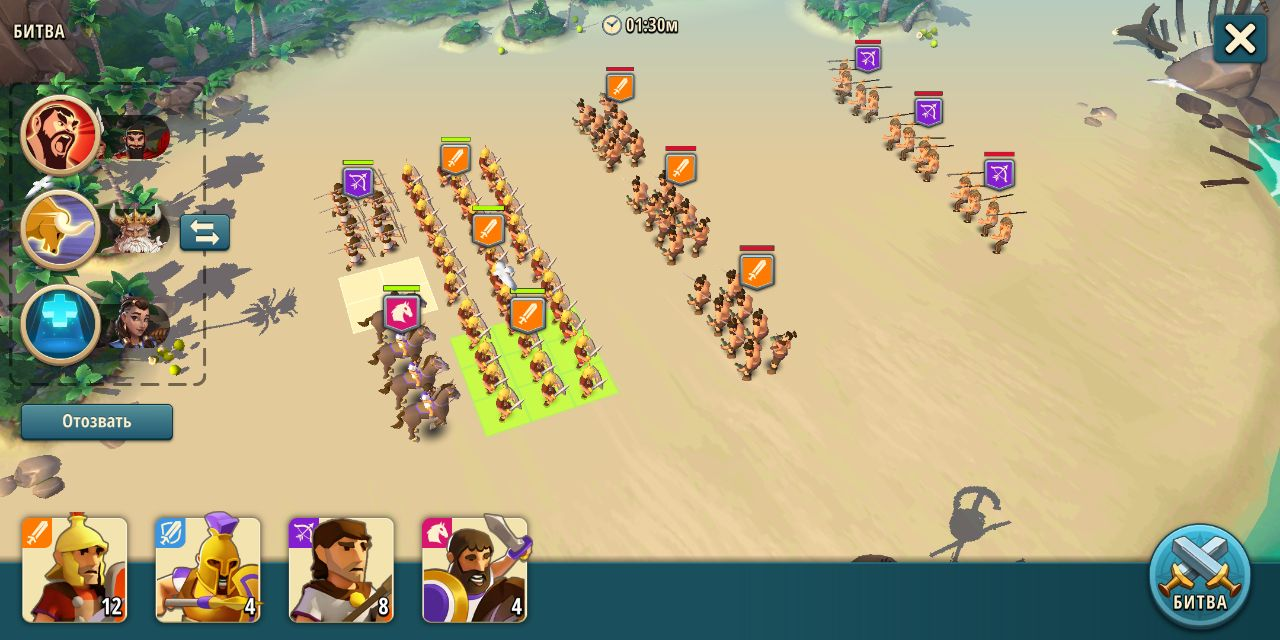
\includegraphics[width=\linewidth]{./parts/media/TreasureHunt/21/sargon/photo_2022-04-06_18-11-33.jpg} \newline
\noindent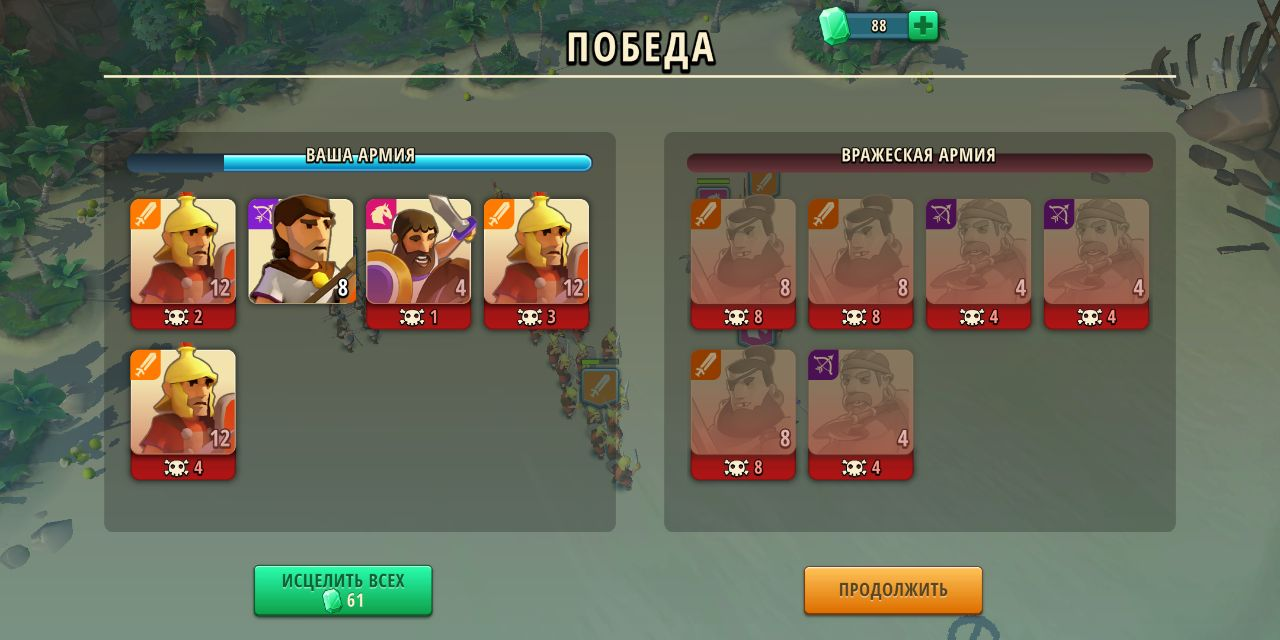
\includegraphics[width=\linewidth]{./parts/media/TreasureHunt/21/sargon/photo_2022-04-06_18-11-59.jpg} \newline

\newpage
\begin{center}
	\hypertarget{fight22}{\textbf{Битва 22 (Sargon).}}
\end{center}
\noindent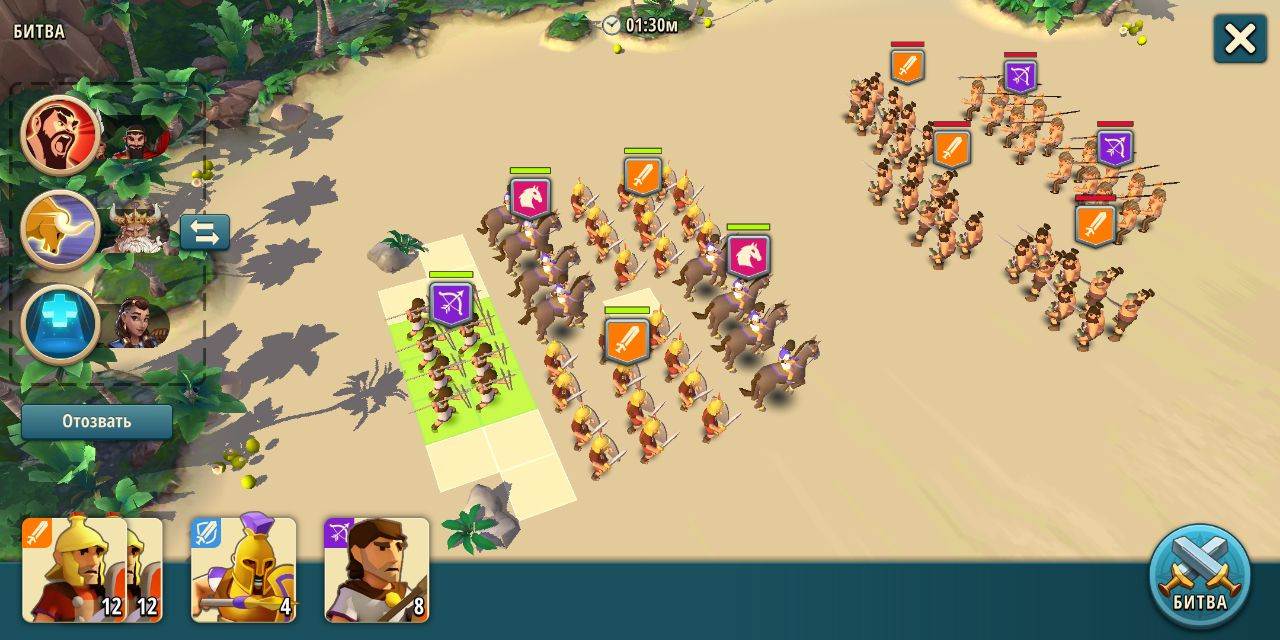
\includegraphics[width=\linewidth]{./parts/media/TreasureHunt/22/sargon/photo_2022-04-06_18-12-03.jpg} \newline
\noindent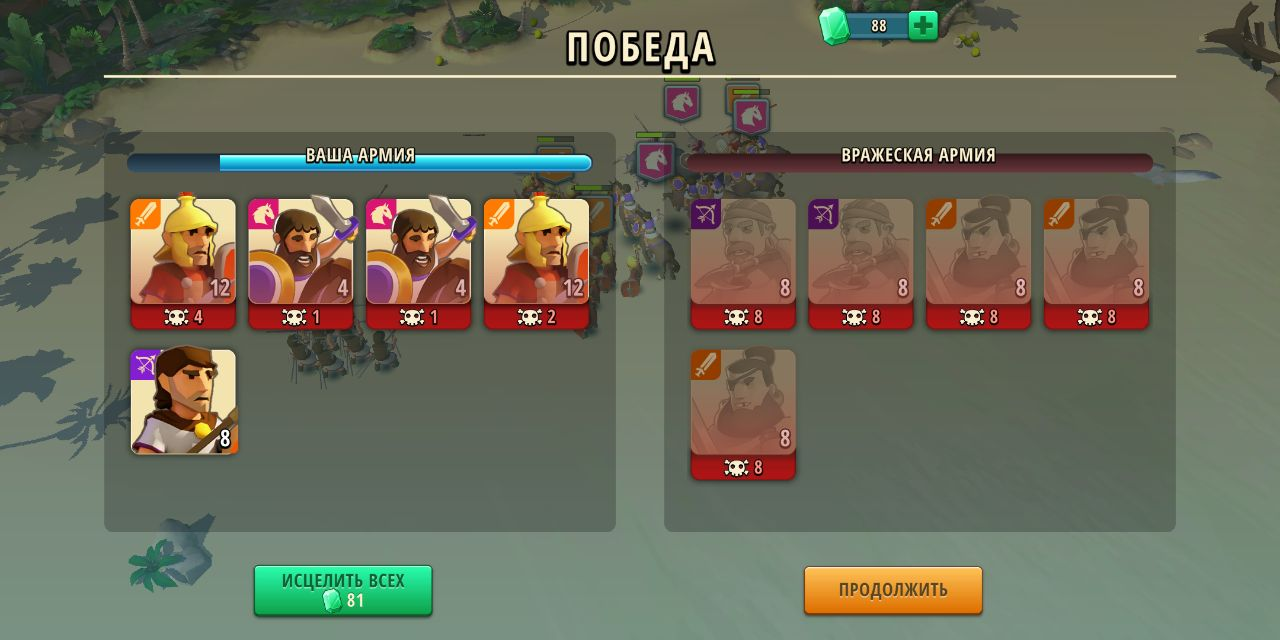
\includegraphics[width=\linewidth]{./parts/media/TreasureHunt/22/sargon/photo_2022-04-06_18-12-13.jpg} \newline

\newpage
\begin{center}
	\hypertarget{fight23}{\textbf{Битва 23 (Sargon).}}
\end{center}
\noindent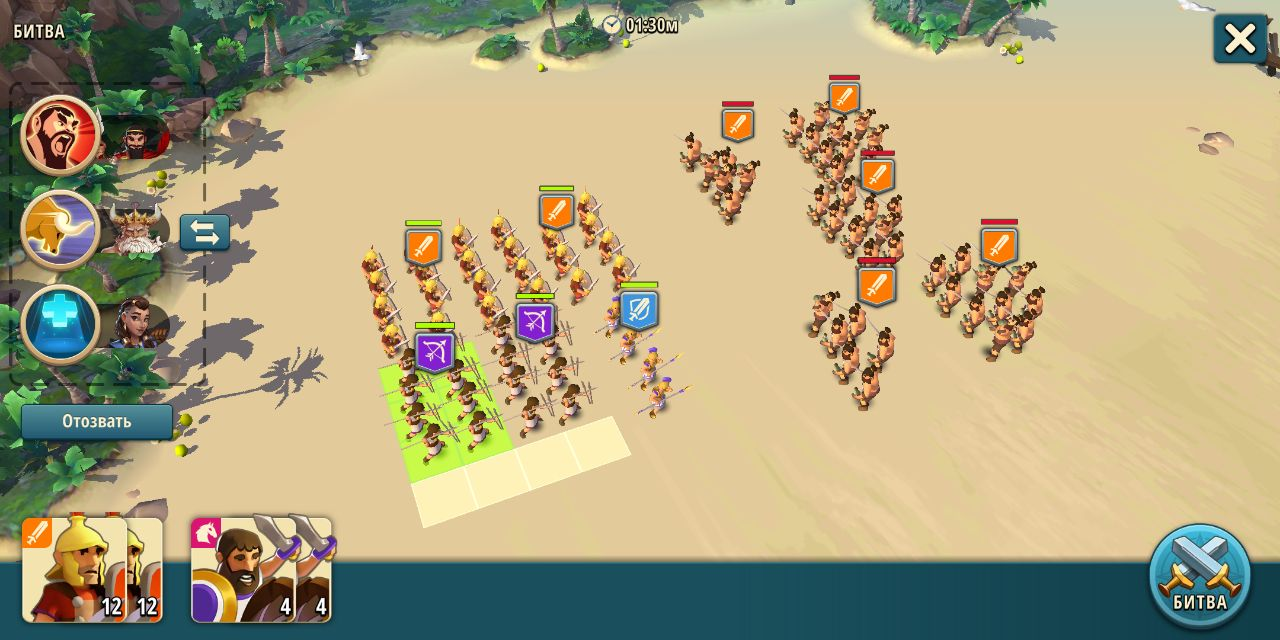
\includegraphics[width=\linewidth]{./parts/media/TreasureHunt/23/sargon/photo_2022-04-06_18-12-18.jpg} \newline
\noindent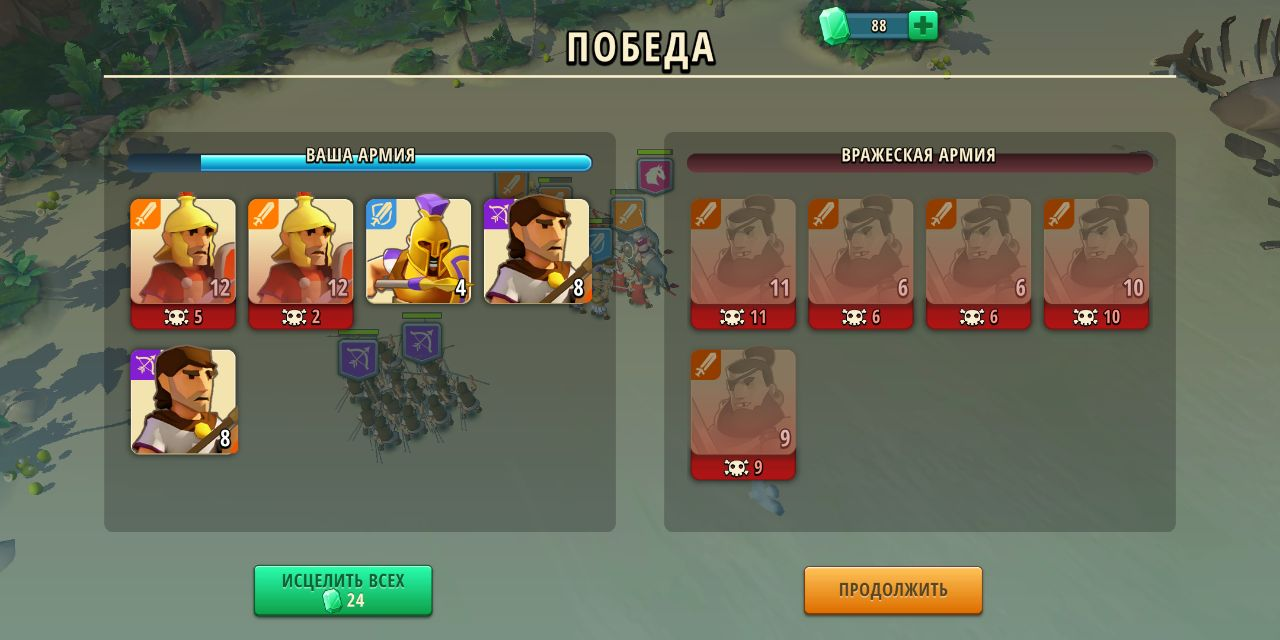
\includegraphics[width=\linewidth]{./parts/media/TreasureHunt/23/sargon/photo_2022-04-06_18-12-26.jpg} \newline

\newpage
\begin{center}
	\hypertarget{fight24}{\textbf{Битва 24 (decoder).}}
\end{center}
\noindent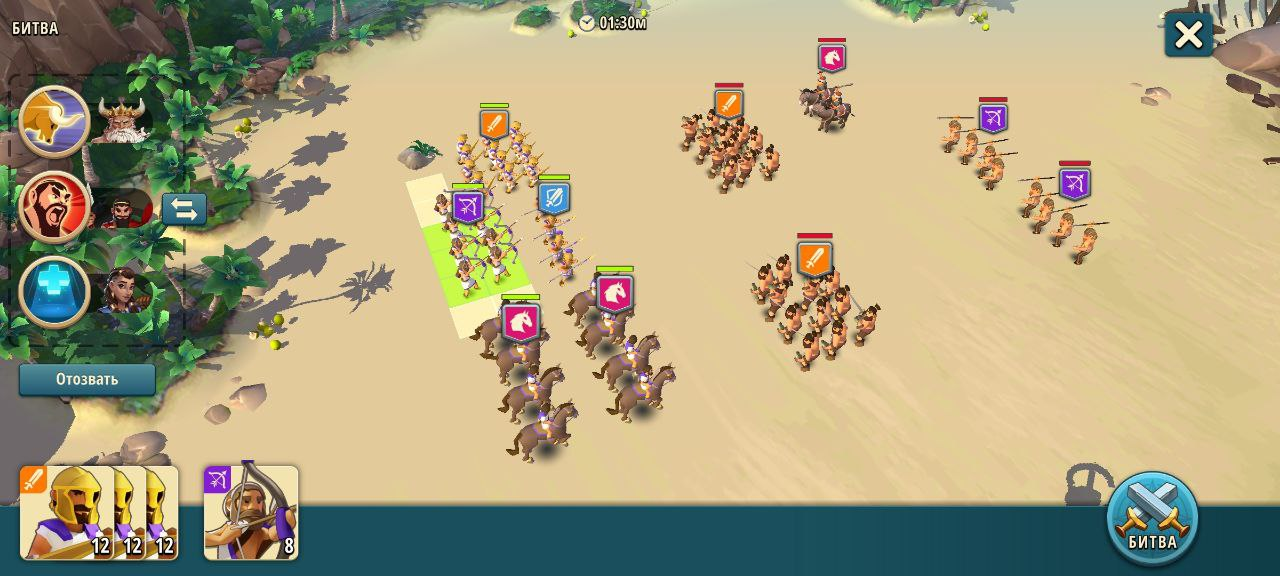
\includegraphics[width=\linewidth]{./parts/media/TreasureHunt/24/decoder/photo_2022-04-06_18-10-02.jpg} \newline
\noindent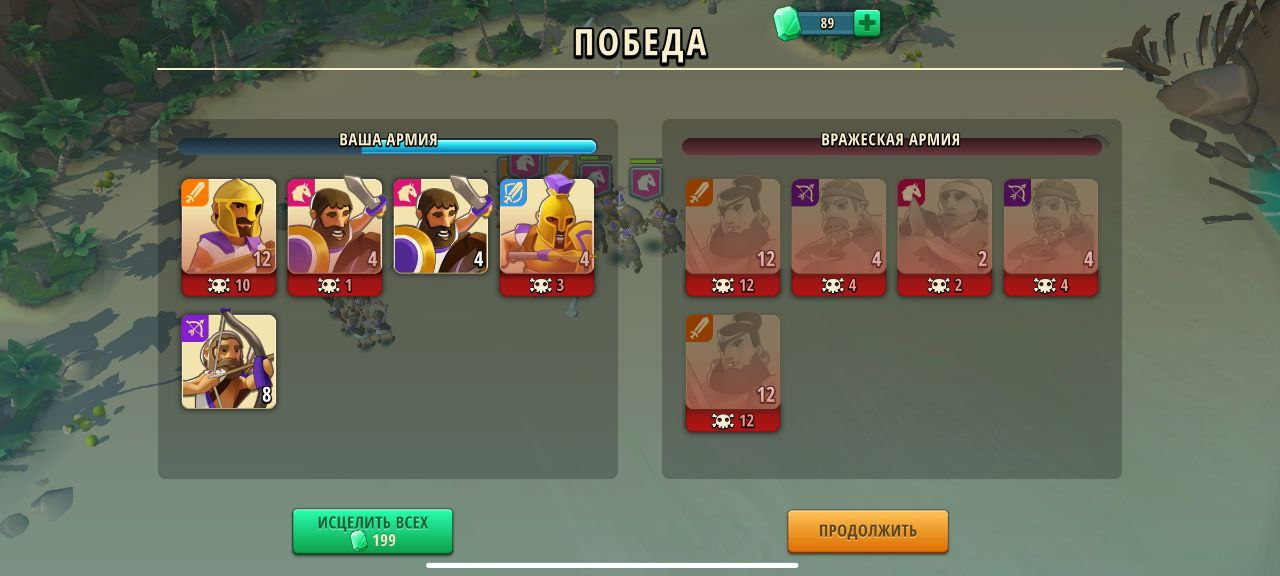
\includegraphics[width=\linewidth]{./parts/media/TreasureHunt/24/decoder/photo_2022-04-06_18-10-13.jpg} \newline

\newpage
\begin{center}
	\hypertarget{fight25}{\textbf{Битва 25 (decoder).}}
\end{center}
\noindent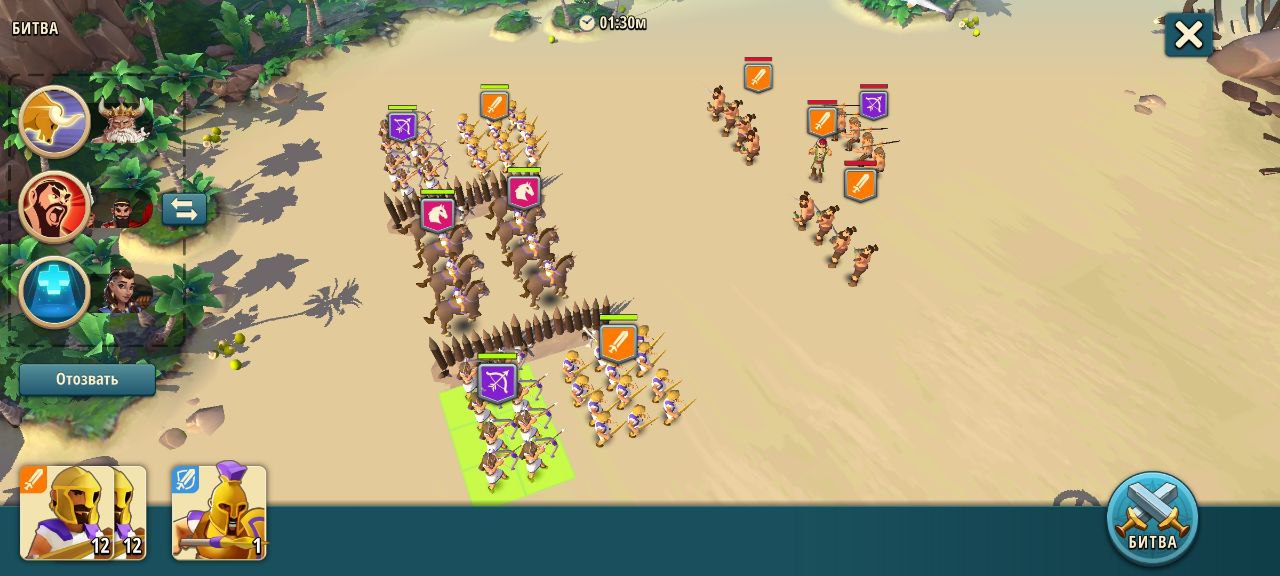
\includegraphics[width=\linewidth]{./parts/media/TreasureHunt/25/decoder/photo_2022-04-13_16-38-30.jpg} \newline
\noindent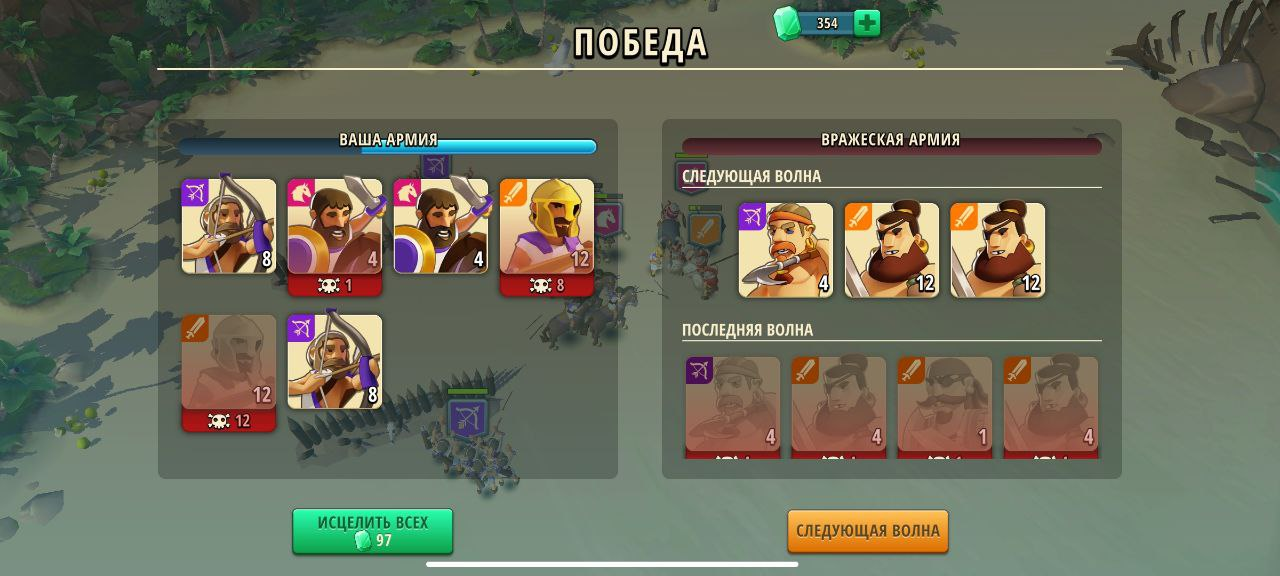
\includegraphics[width=\linewidth]{./parts/media/TreasureHunt/25/decoder/photo_2022-04-13_16-38-45.jpg} \newline
\noindent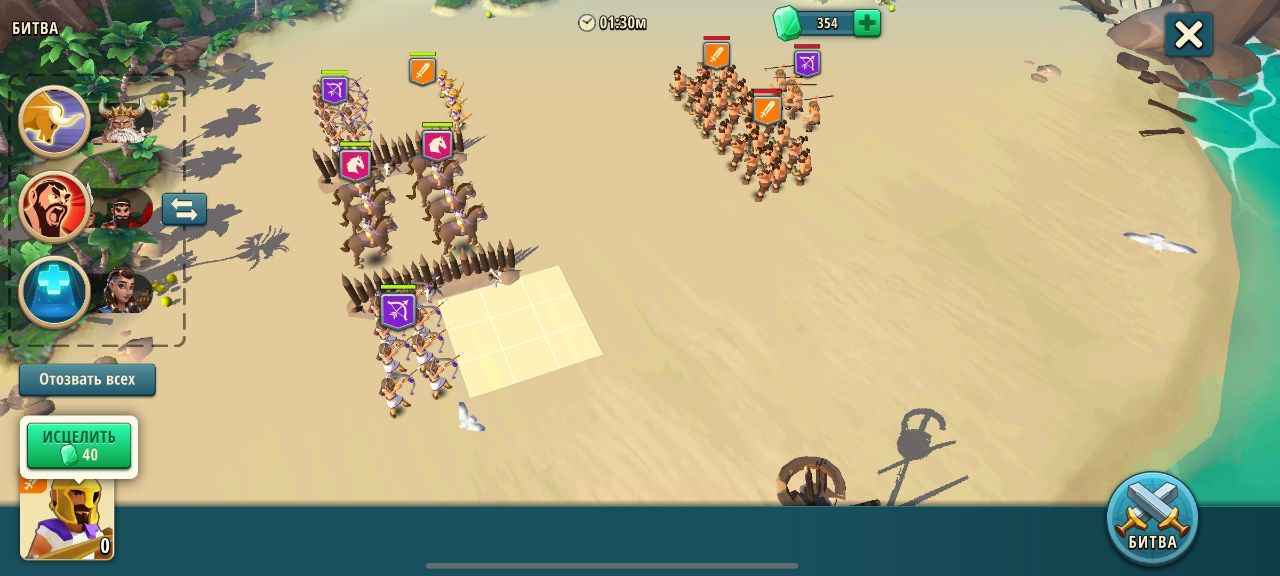
\includegraphics[width=\linewidth]{./parts/media/TreasureHunt/25/decoder/photo_2022-04-13_16-38-53.jpg} \newline
\noindent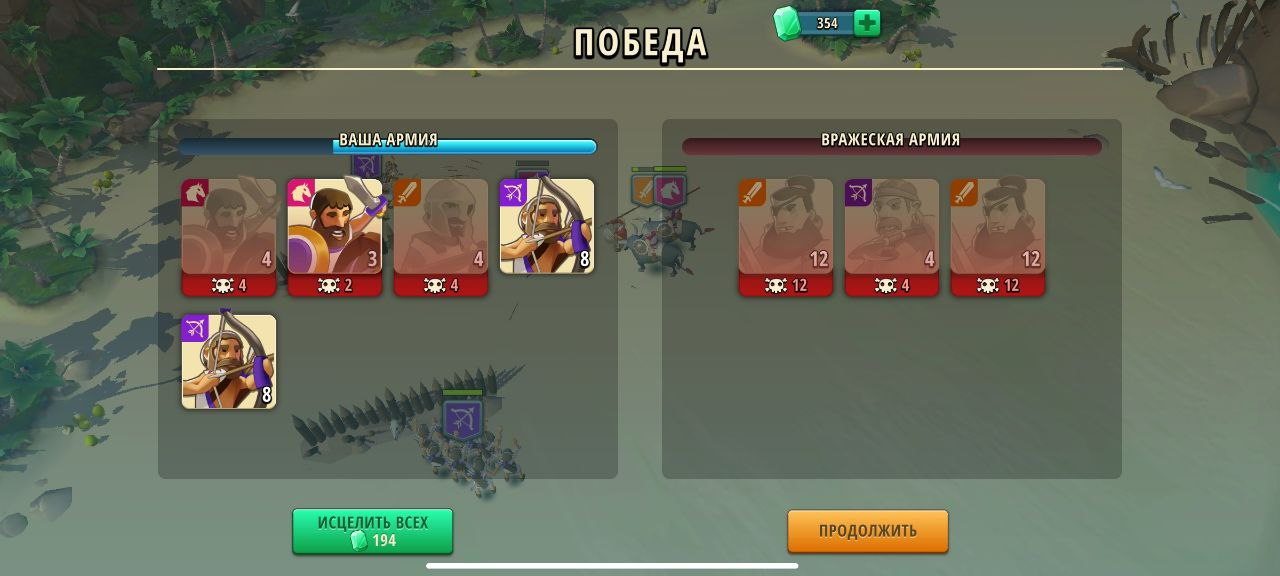
\includegraphics[width=\linewidth]{./parts/media/TreasureHunt/25/decoder/photo_2022-04-13_16-38-58.jpg} \newline

\newpage
\begin{center}
	\hypertarget{fight26}{\textbf{Битва 26 (decoder).}}
\end{center}
\noindent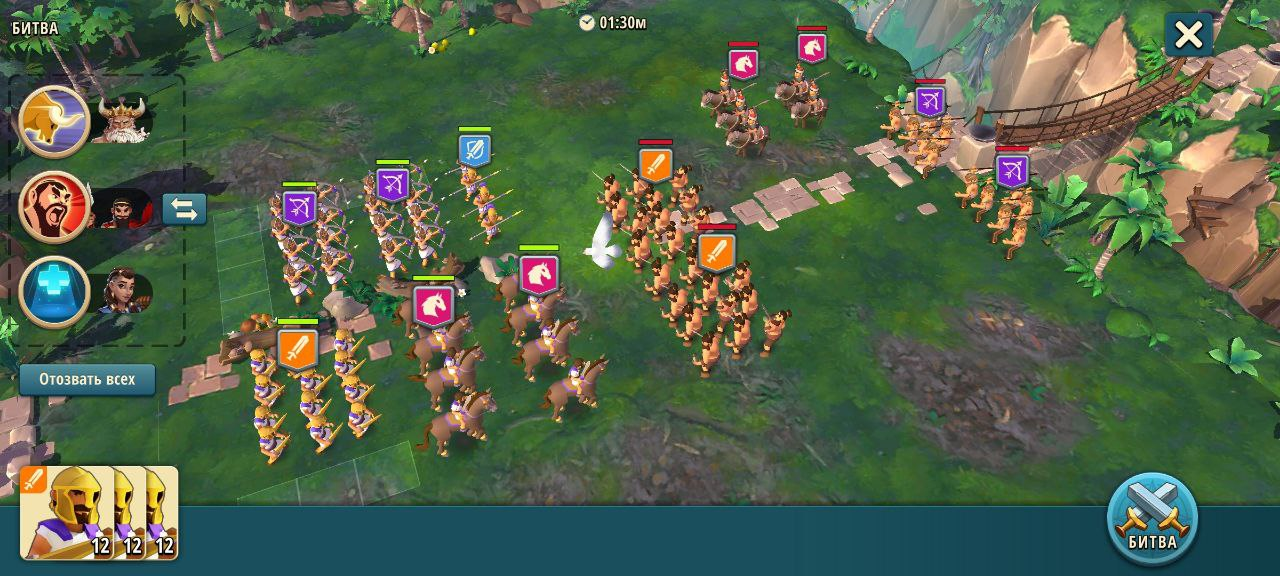
\includegraphics[width=\linewidth]{./parts/media/TreasureHunt/26/decoder/photo_2022-04-06_18-11-14.jpg} \newline
\noindent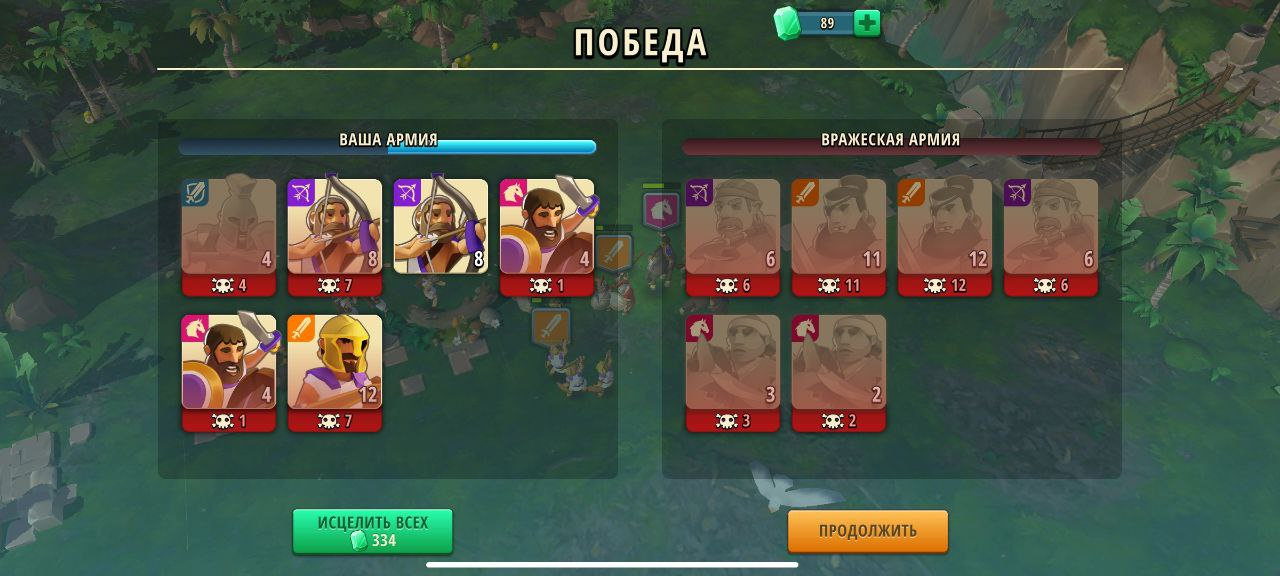
\includegraphics[width=\linewidth]{./parts/media/TreasureHunt/26/decoder/photo_2022-04-06_18-11-23.jpg} \newline

\newpage
\begin{center}
	\hypertarget{fight27}{\textbf{Битва 27 (decoder).}}
\end{center}
\noindent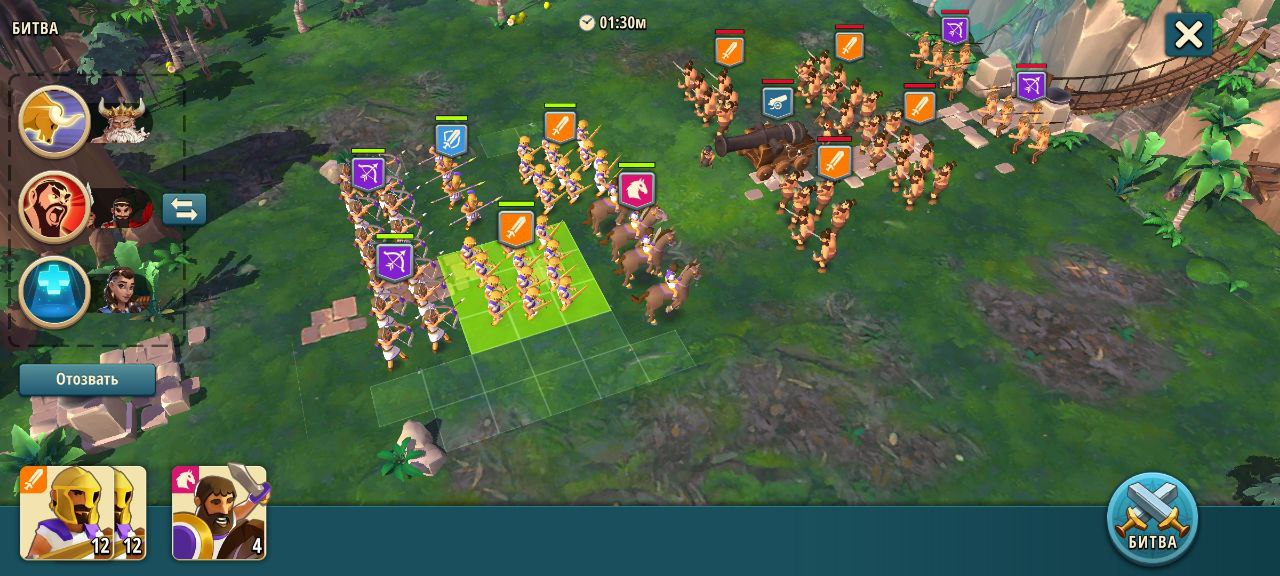
\includegraphics[width=\linewidth]{./parts/media/TreasureHunt/27/decoder/photo_2022-04-13_17-26-43.jpg} \newline
\noindent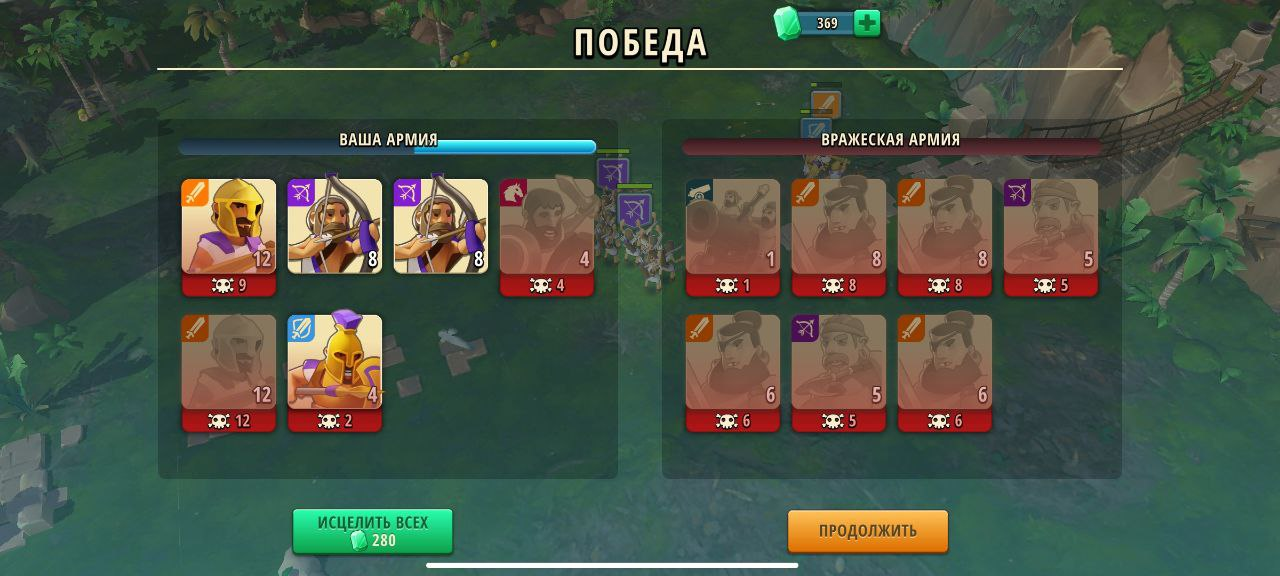
\includegraphics[width=\linewidth]{./parts/media/TreasureHunt/27/decoder/photo_2022-04-13_17-27-02.jpg} \newline

\newpage
\begin{center}
	\hypertarget{fight28}{\textbf{Битва 28 (Preyton).}}
\end{center}
\noindent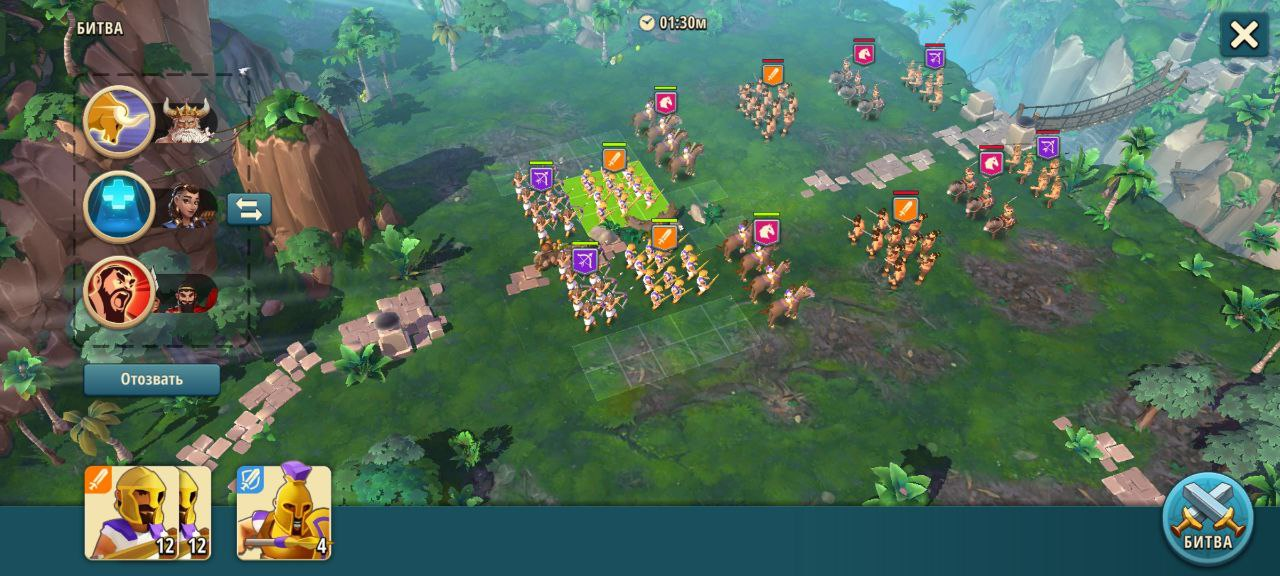
\includegraphics[width=\linewidth]{./parts/media/TreasureHunt/28/Preyton/28.jpg} \newline
\noindent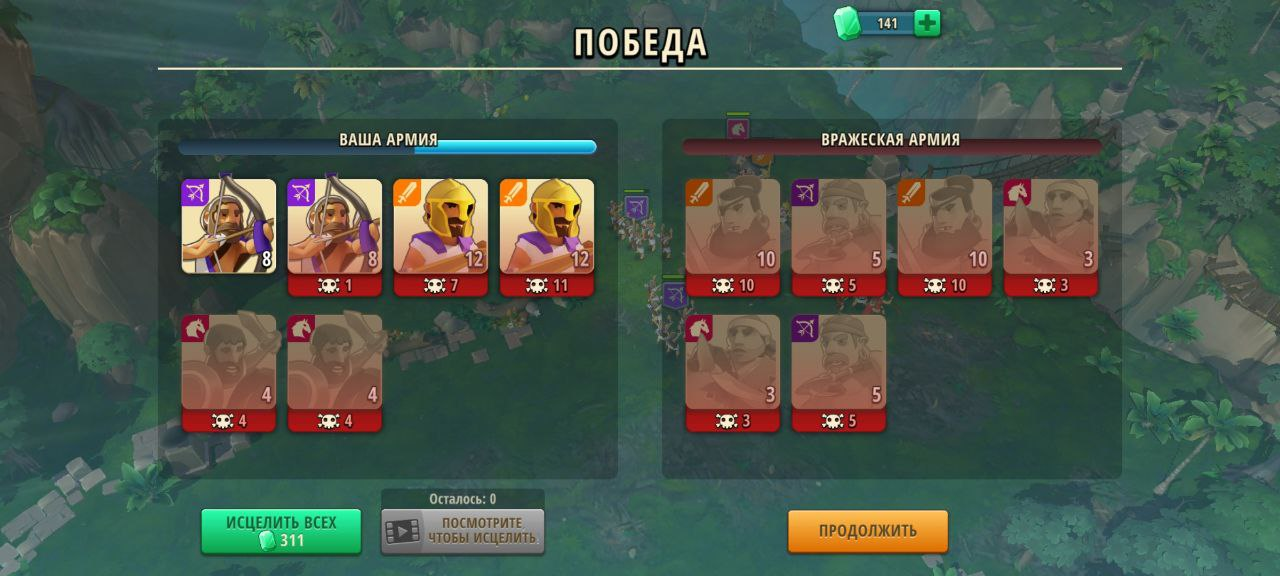
\includegraphics[width=\linewidth]{./parts/media/TreasureHunt/28/Preyton/28..jpg} \newline

\newpage
\begin{center}
	\hypertarget{fight29}{\textbf{Битва 29 (Preyton).}}
\end{center}
\noindent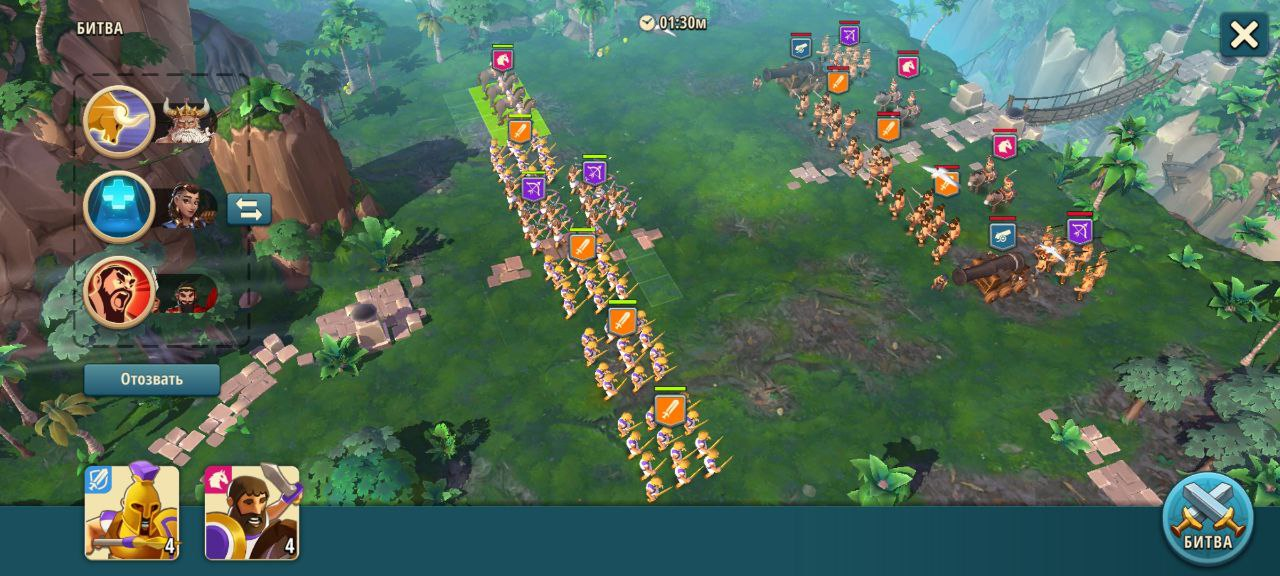
\includegraphics[width=\linewidth]{./parts/media/TreasureHunt/29/Preyton/29.jpg} \newline
\noindent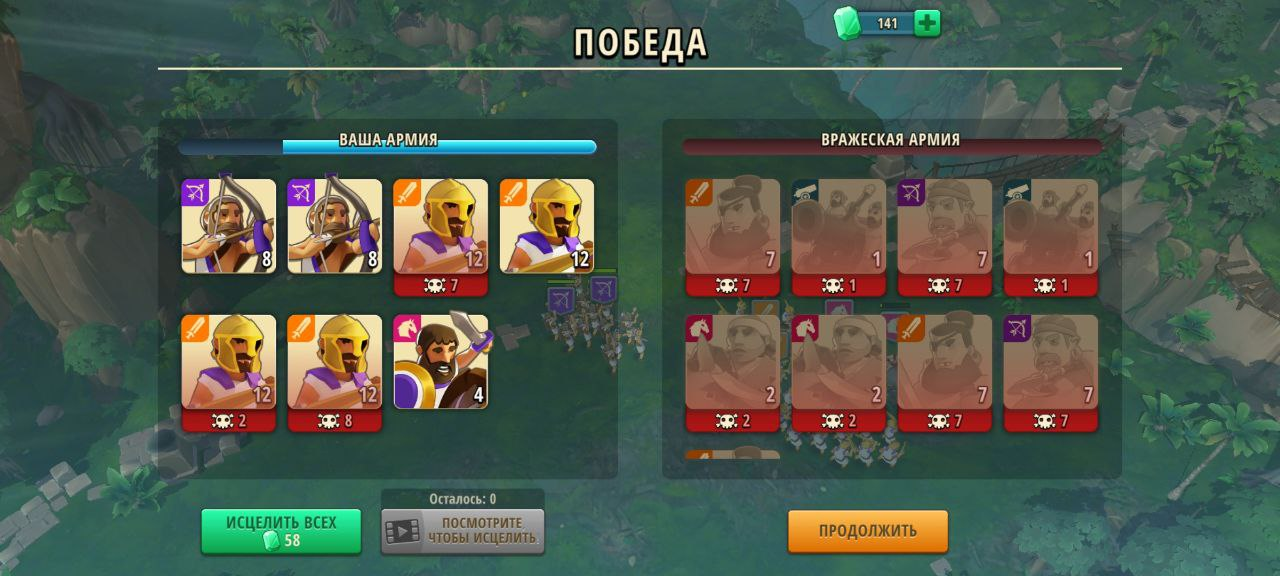
\includegraphics[width=\linewidth]{./parts/media/TreasureHunt/29/Preyton/29..jpg} \newline

\newpage
\begin{center}
	\hypertarget{fight30}{\textbf{Битва 30 (decoder).}}
\end{center}
\noindent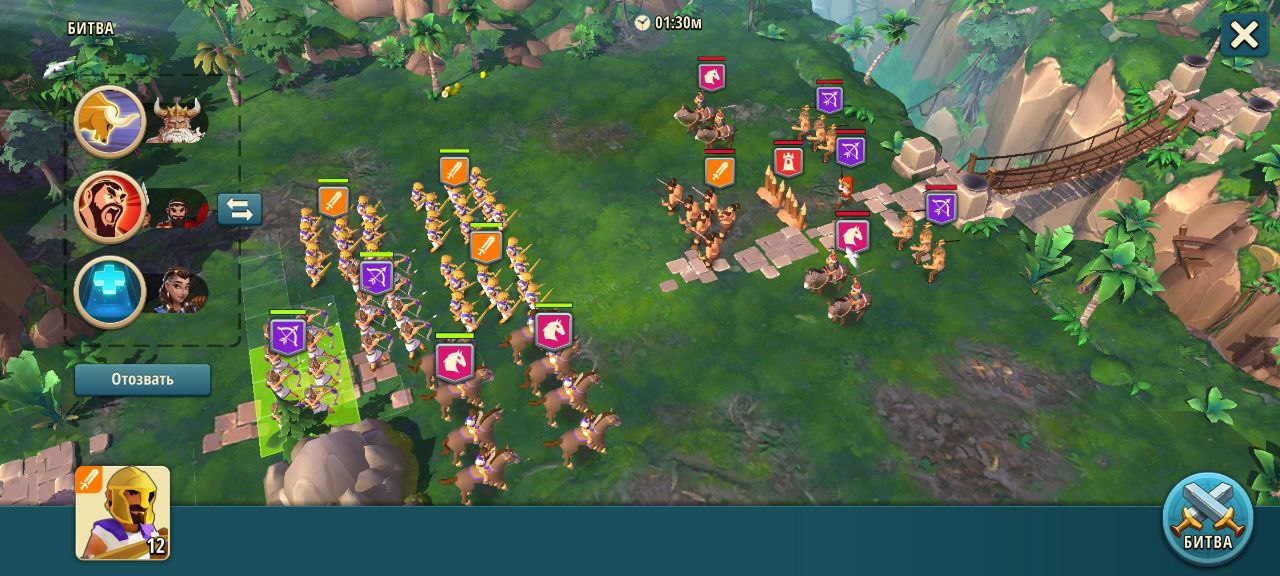
\includegraphics[width=\linewidth]{./parts/media/TreasureHunt/30/decoder/photo_2022-04-07_09-59-28.jpg} \newline
\noindent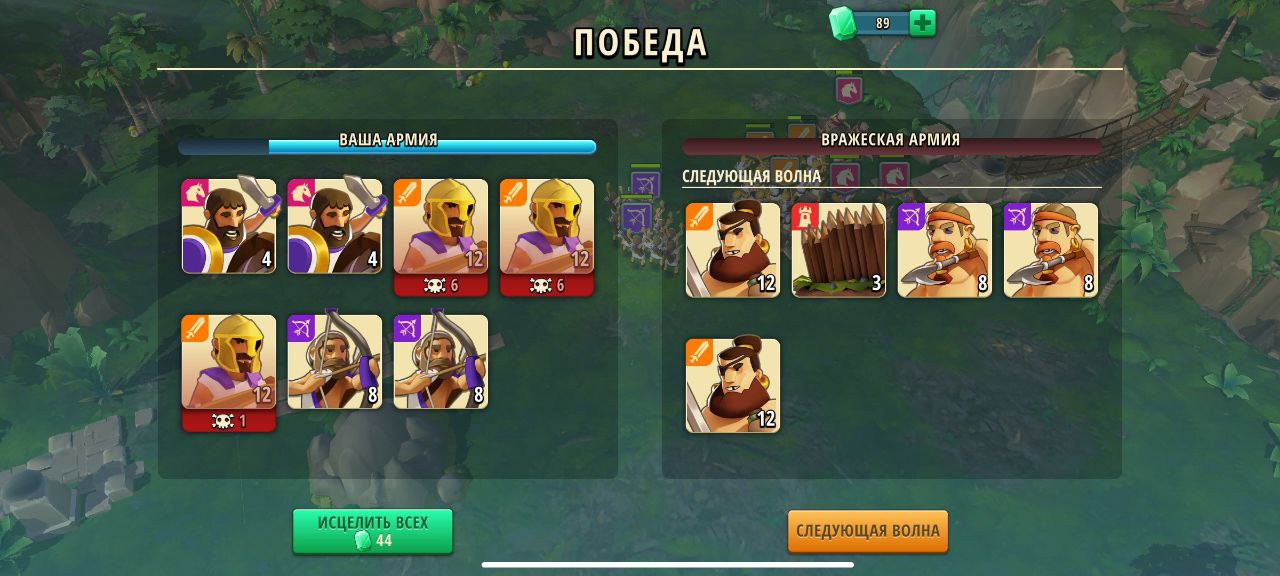
\includegraphics[width=\linewidth]{./parts/media/TreasureHunt/30/decoder/photo_2022-04-07_09-59-40.jpg} \newline
\noindent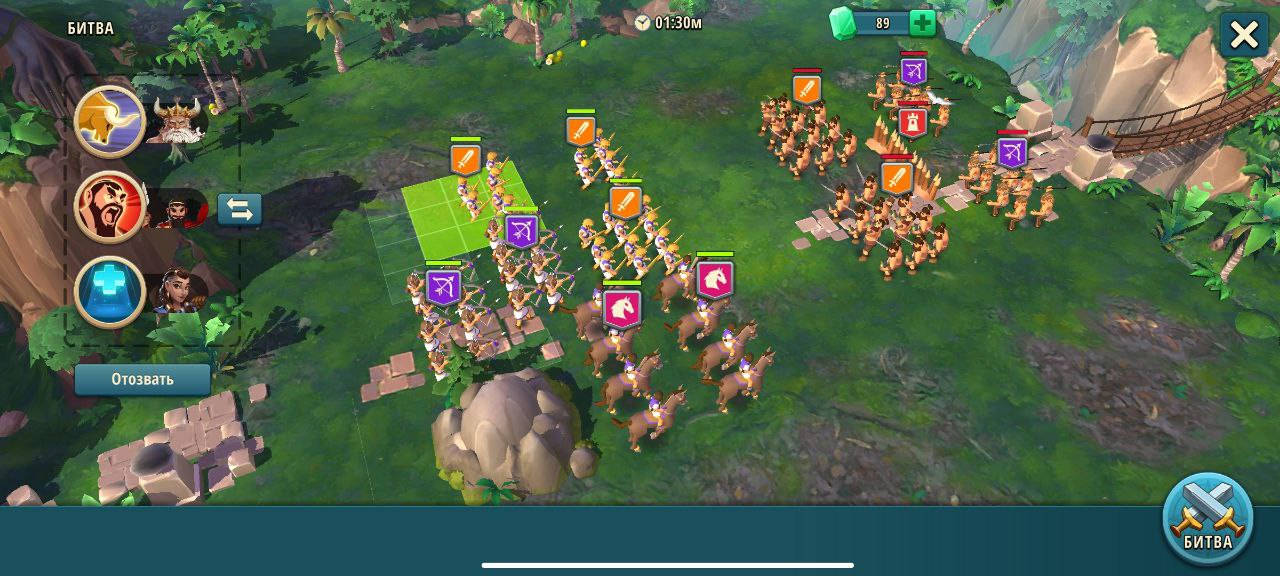
\includegraphics[width=\linewidth]{./parts/media/TreasureHunt/30/decoder/photo_2022-04-07_10-00-22.jpg} \newline
\noindent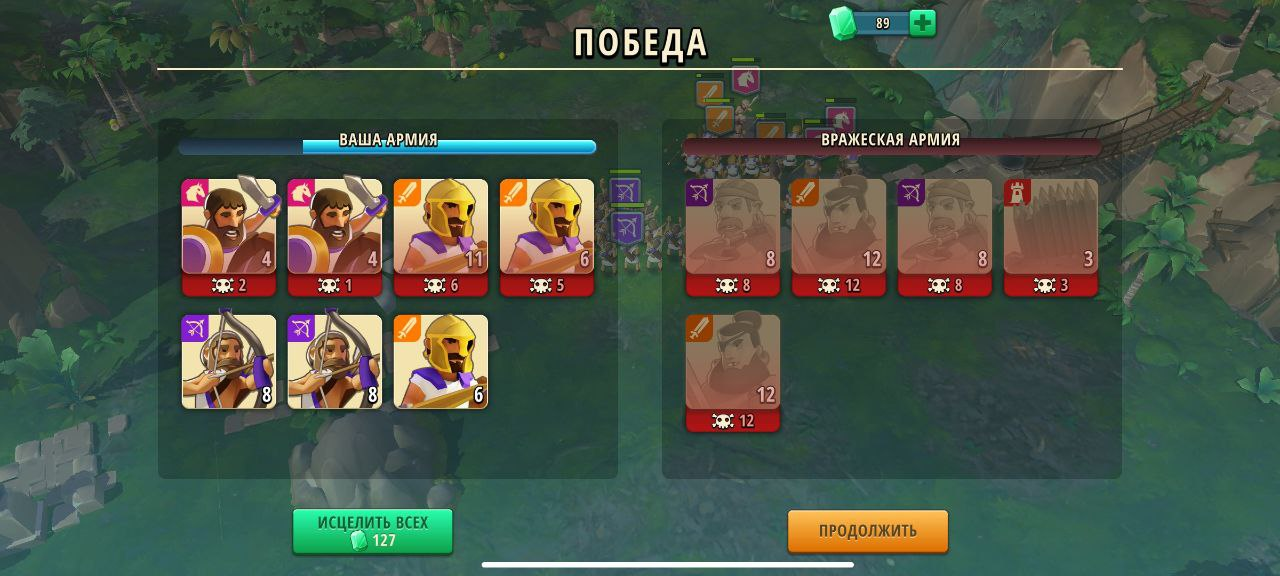
\includegraphics[width=\linewidth]{./parts/media/TreasureHunt/30/decoder/photo_2022-04-07_10-00-32.jpg} \newline

\newpage
\begin{center}
	\hypertarget{fight31}{\textbf{Битва 31 (Sargon).}}
\end{center}
\noindent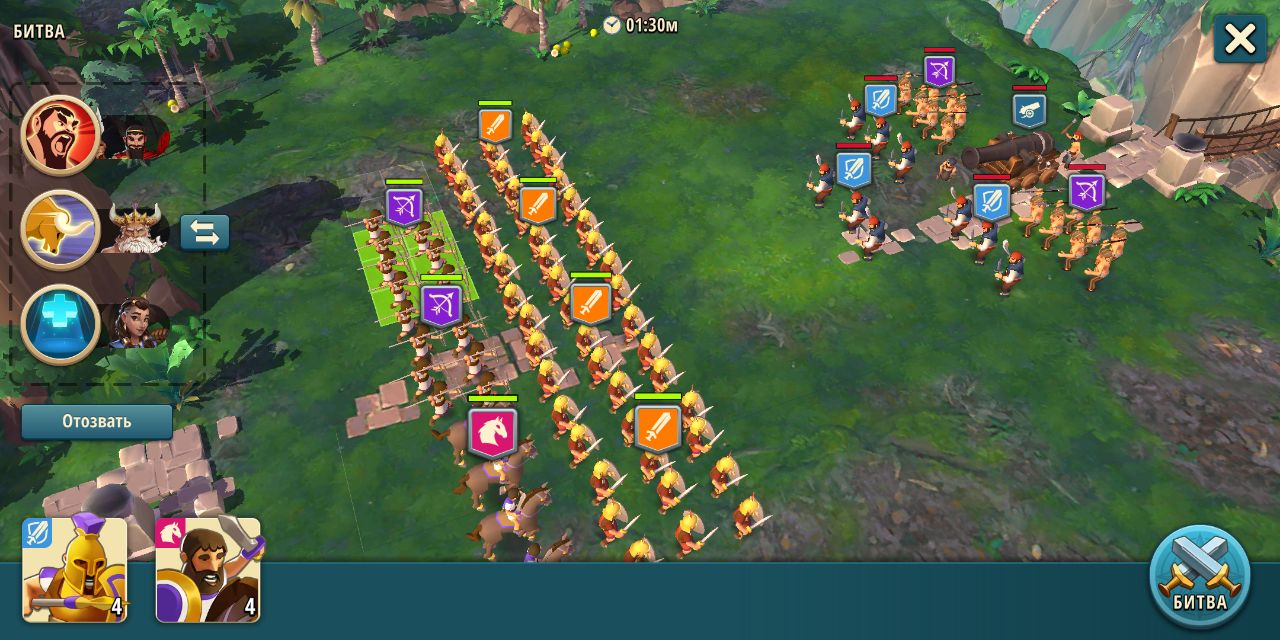
\includegraphics[width=\linewidth]{./parts/media/TreasureHunt/31/sargon/photo_2022-04-07_10-05-08.jpg} \newline
\noindent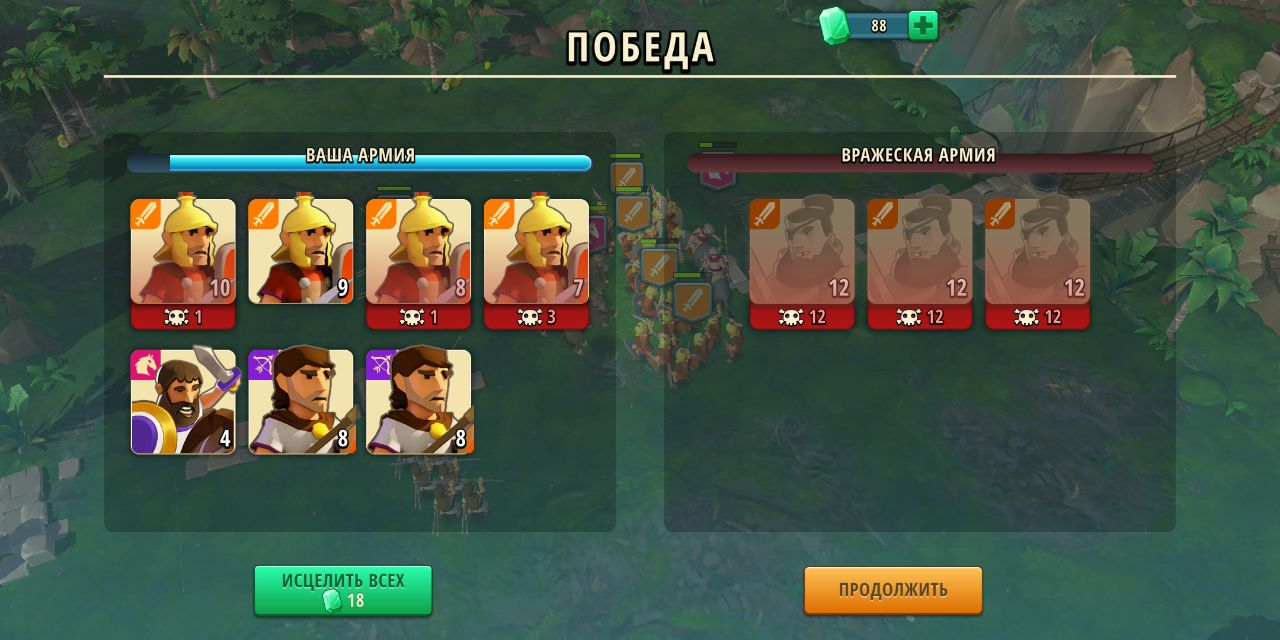
\includegraphics[width=\linewidth]{./parts/media/TreasureHunt/31/sargon/photo_2022-04-07_10-05-25.jpg} \newline
\noindent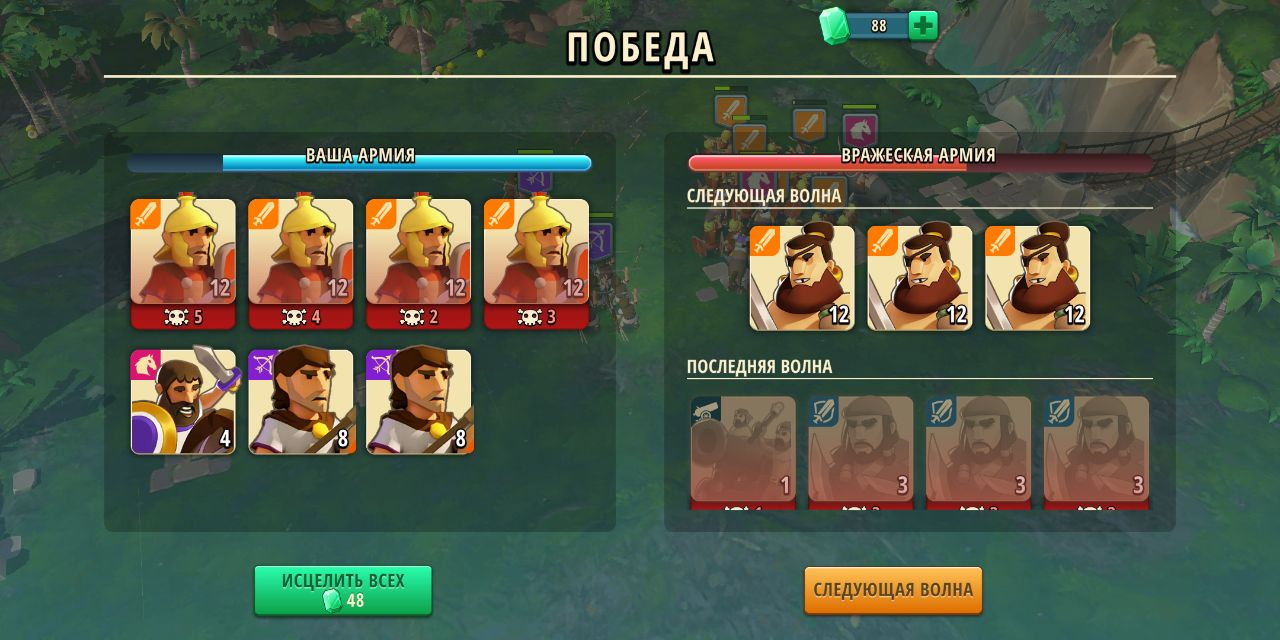
\includegraphics[width=\linewidth]{./parts/media/TreasureHunt/31/sargon/photo_2022-04-07_10-05-18.jpg} \newline
\noindent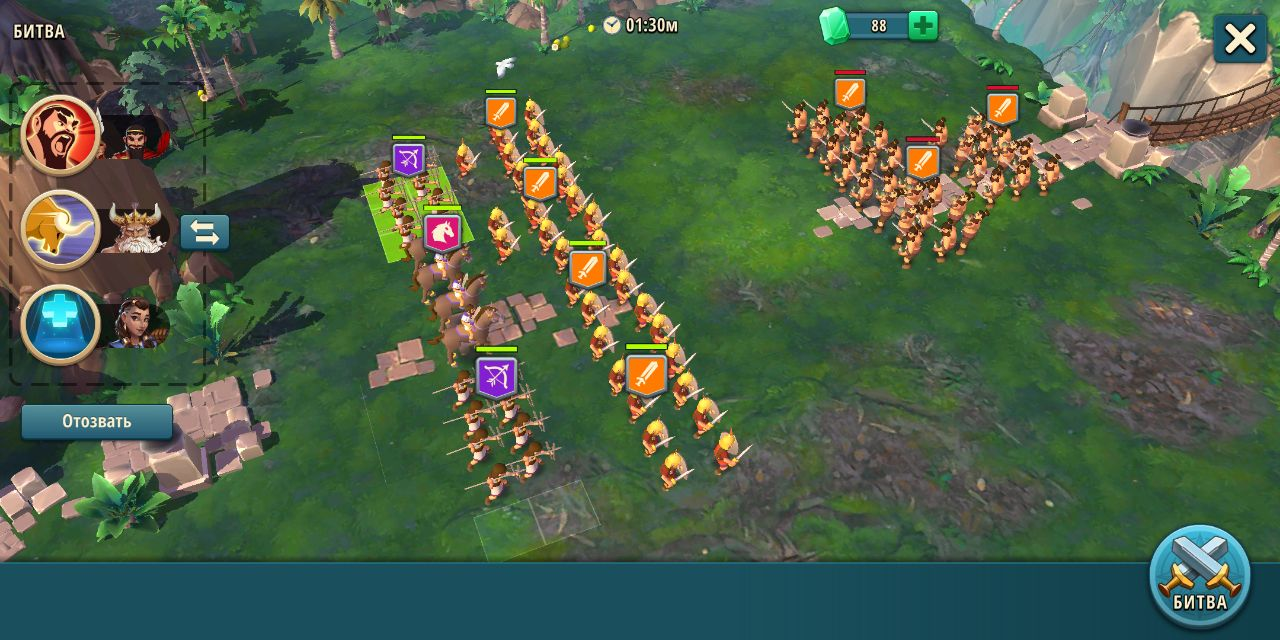
\includegraphics[width=\linewidth]{./parts/media/TreasureHunt/31/sargon/photo_2022-04-07_10-05-22.jpg} \newline

\newpage
\begin{center}
	\hypertarget{fight32}{\textbf{Битва 32 (decoder).}}
\end{center}
\noindent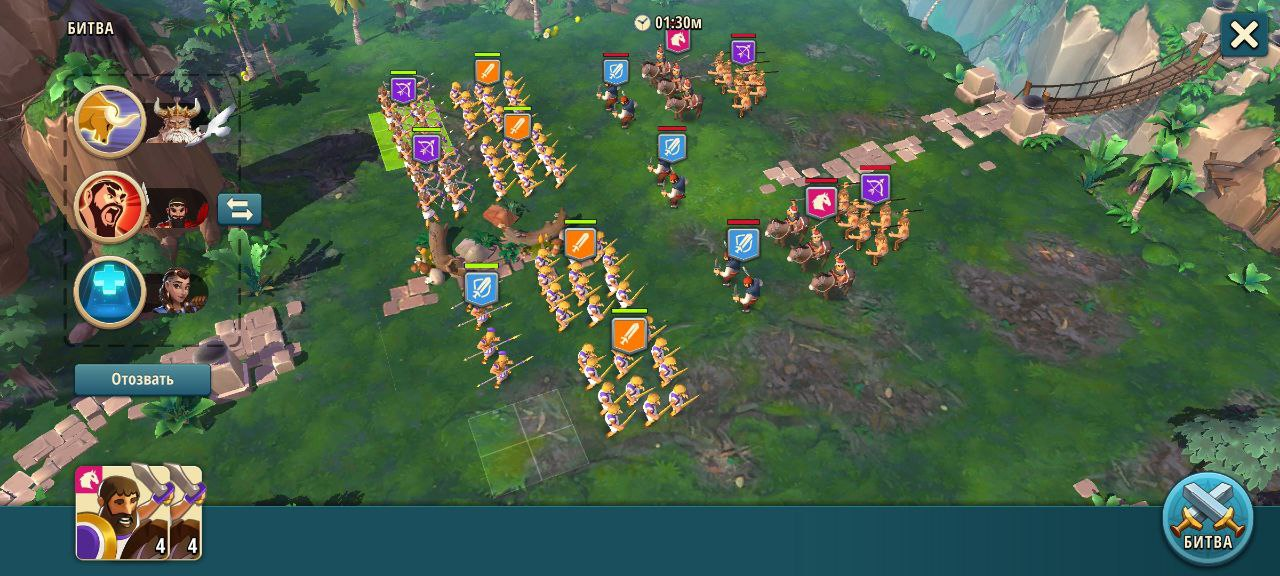
\includegraphics[width=\linewidth]{./parts/media/TreasureHunt/32/decoder/photo_2022-04-07_10-00-59.jpg} \newline
\noindent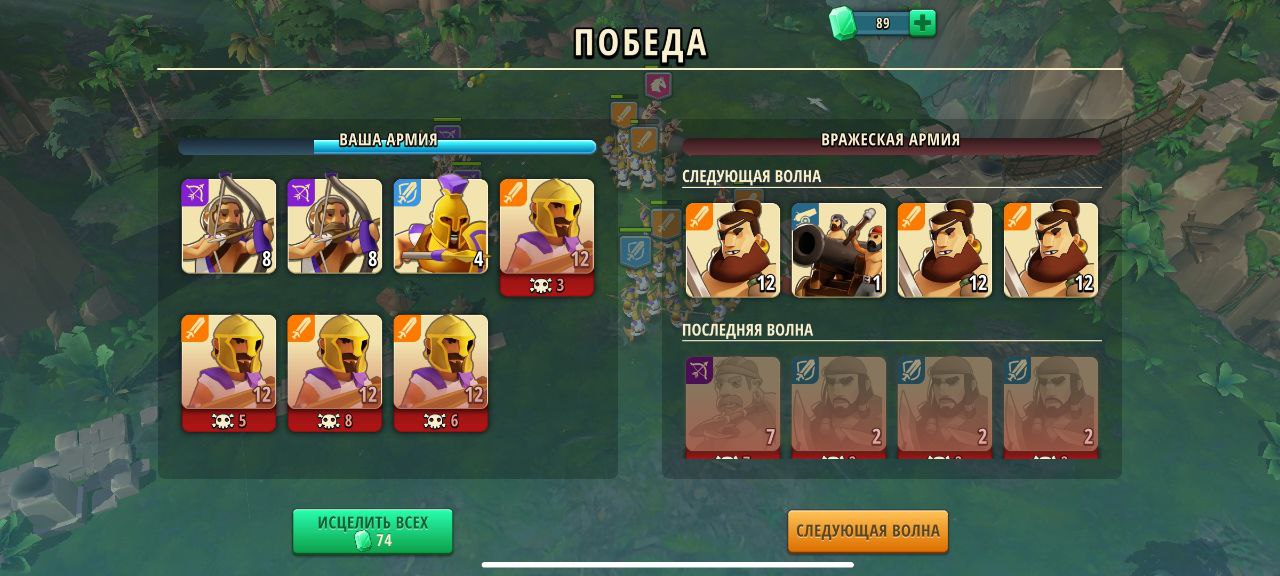
\includegraphics[width=\linewidth]{./parts/media/TreasureHunt/32/decoder/photo_2022-04-07_10-01-48.jpg} \newline
\noindent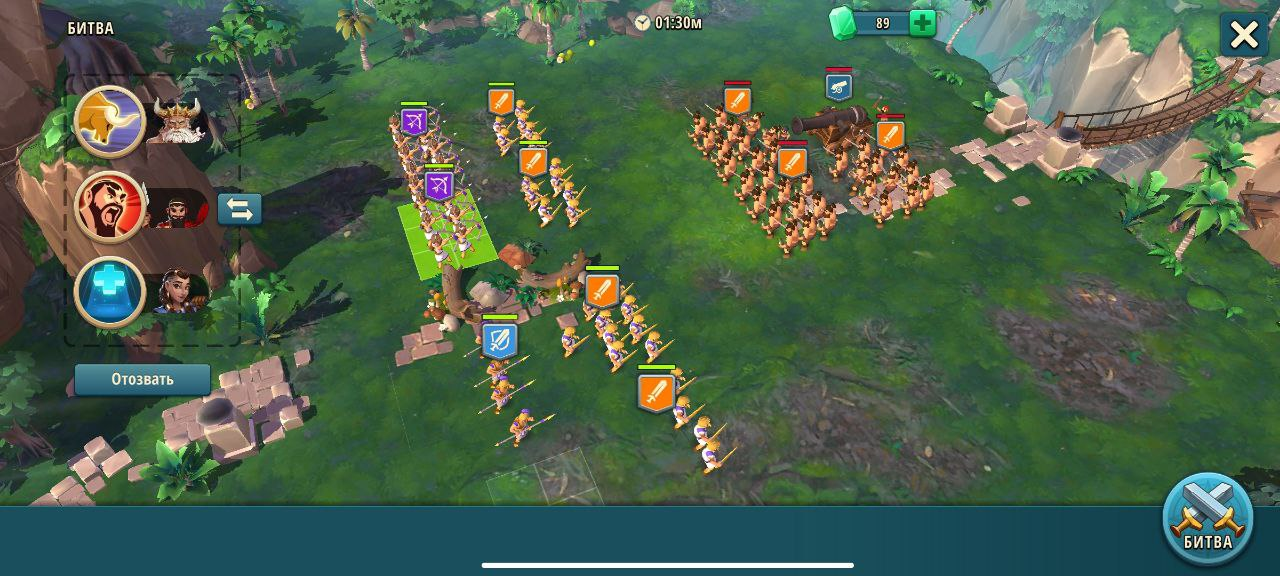
\includegraphics[width=\linewidth]{./parts/media/TreasureHunt/32/decoder/photo_2022-04-07_10-01-54.jpg} \newline
\noindent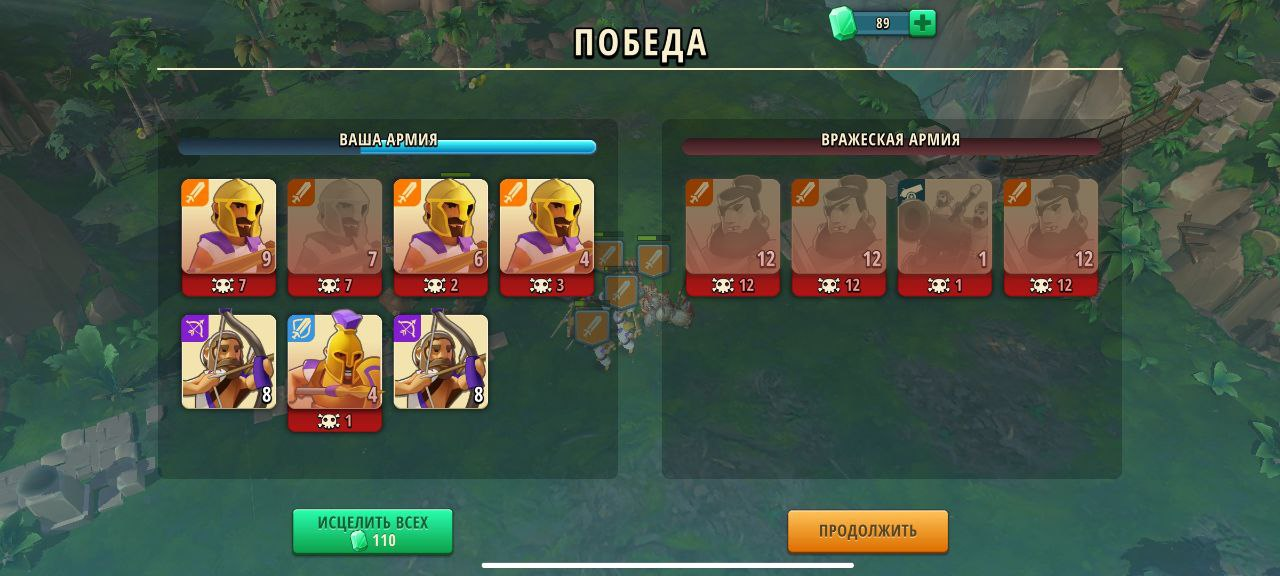
\includegraphics[width=\linewidth]{./parts/media/TreasureHunt/32/decoder/photo_2022-04-07_10-01-57.jpg} \newline

\newpage
\begin{center}
	\hypertarget{fight33}{\textbf{Битва 33 (Sargon).}}
\end{center}
\noindent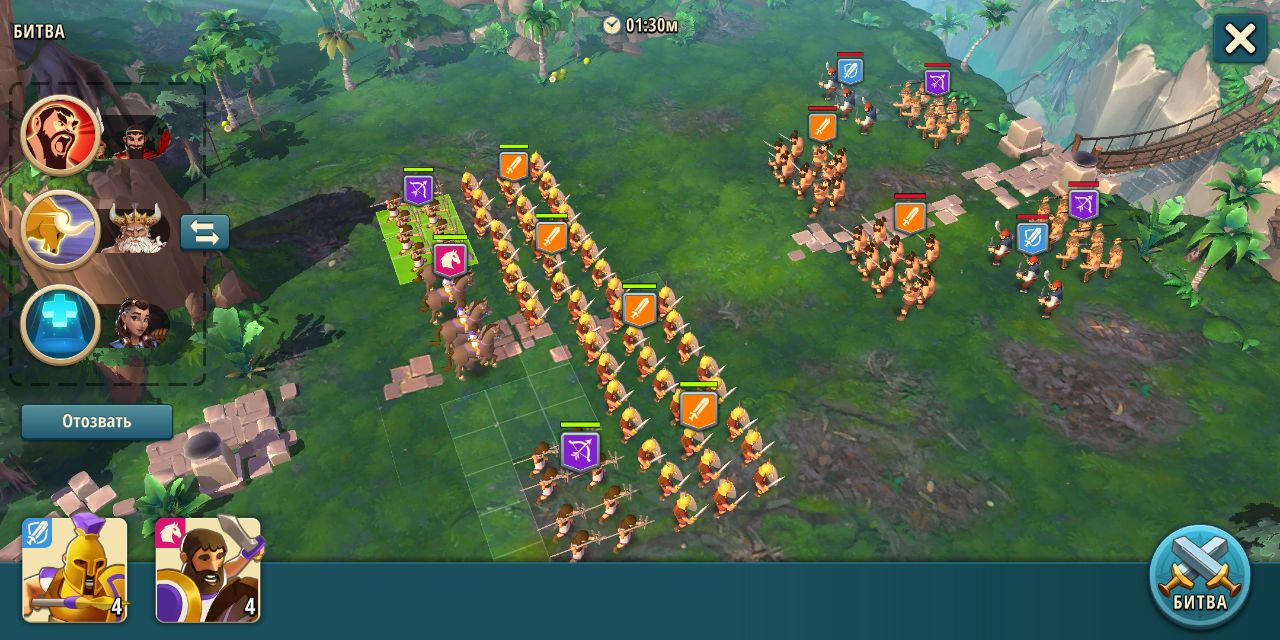
\includegraphics[width=\linewidth]{./parts/media/TreasureHunt/33/sargon/photo_2022-04-07_10-06-22.jpg} \newline
\noindent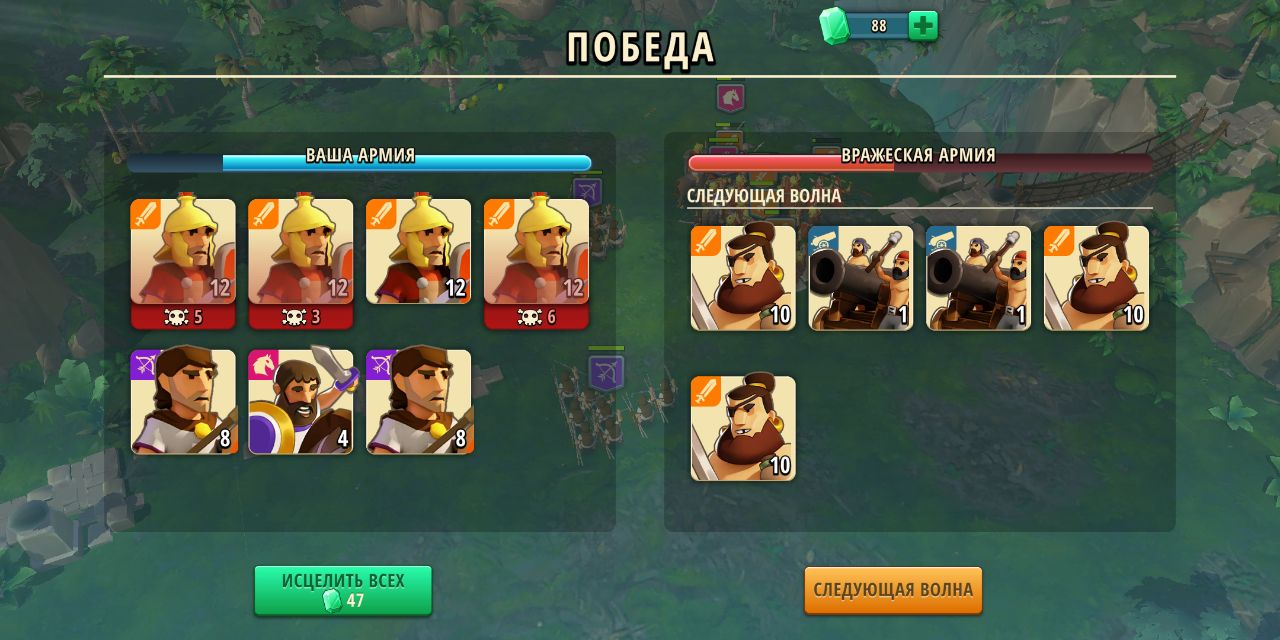
\includegraphics[width=\linewidth]{./parts/media/TreasureHunt/33/sargon/photo_2022-04-07_10-06-34.jpg} \newline
\noindent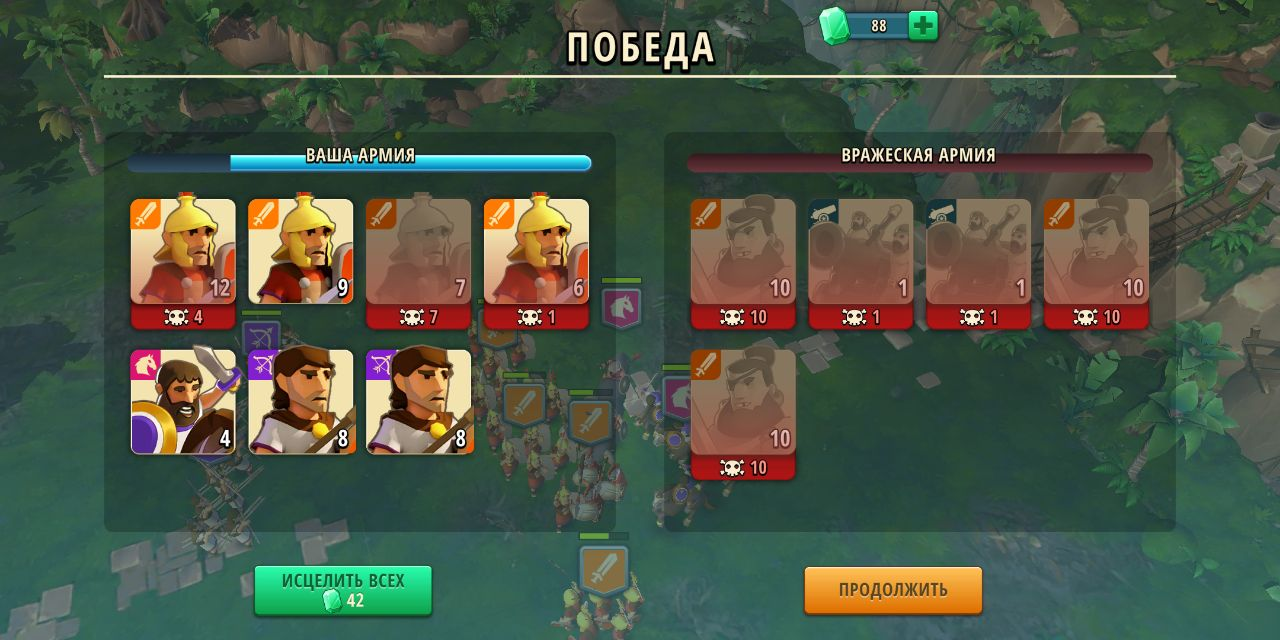
\includegraphics[width=\linewidth]{./parts/media/TreasureHunt/33/sargon/photo_2022-04-07_10-06-40.jpg} \newline
\noindent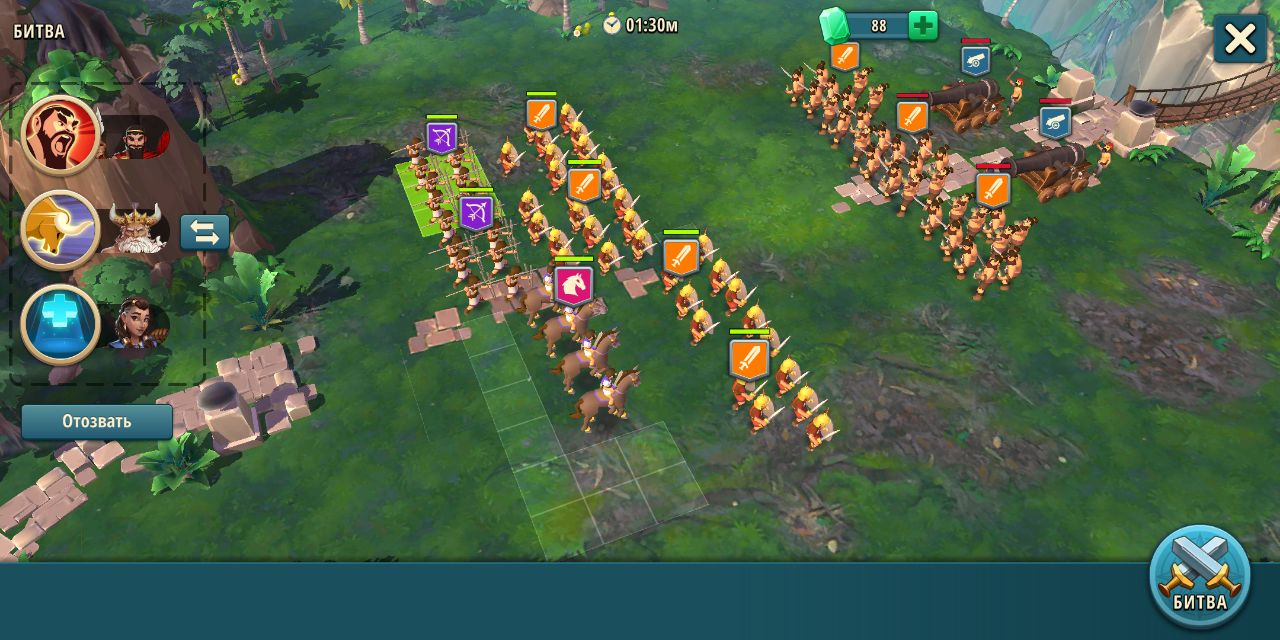
\includegraphics[width=\linewidth]{./parts/media/TreasureHunt/33/sargon/photo_2022-04-07_10-06-37.jpg} \newline

\newpage
\begin{center}
	\hypertarget{fight34}{\textbf{Битва 34 (decoder).}}
\end{center}
\noindent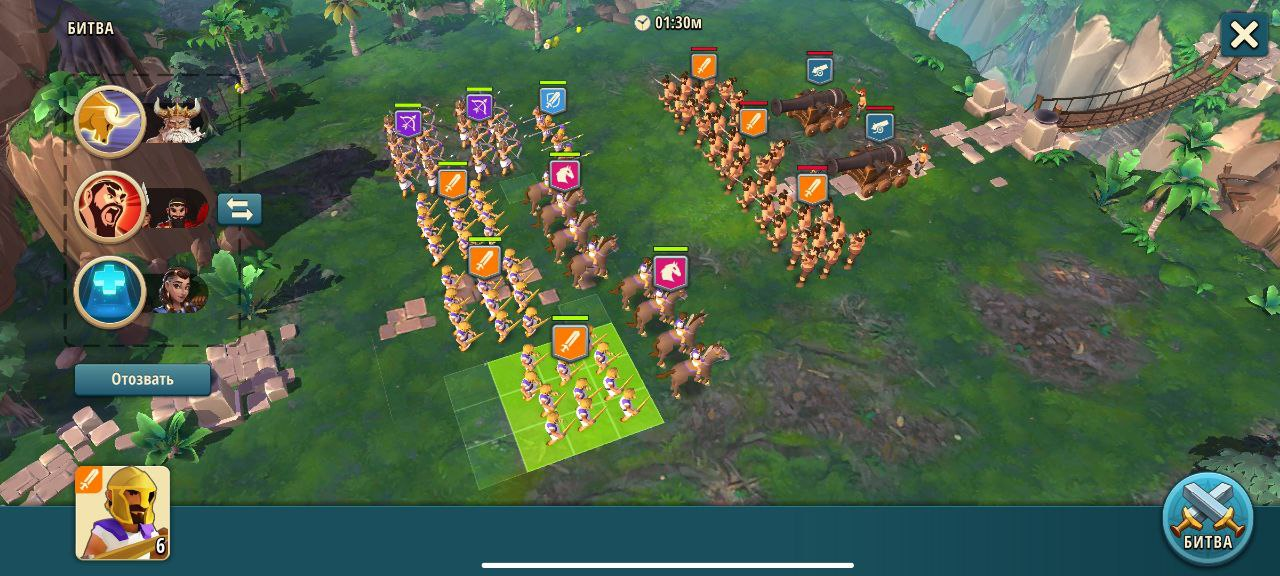
\includegraphics[width=\linewidth]{./parts/media/TreasureHunt/34/decoder/photo_2022-04-07_10-02-34.jpg} \newline
\noindent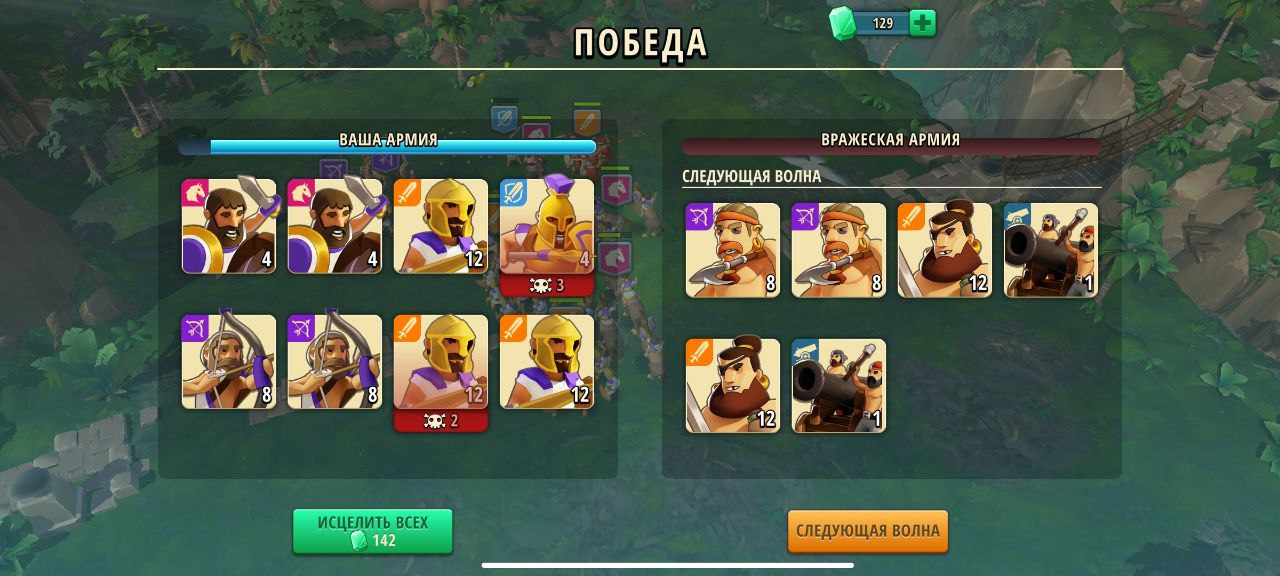
\includegraphics[width=\linewidth]{./parts/media/TreasureHunt/34/decoder/photo_2022-04-07_10-02-43.jpg} \newline
\noindent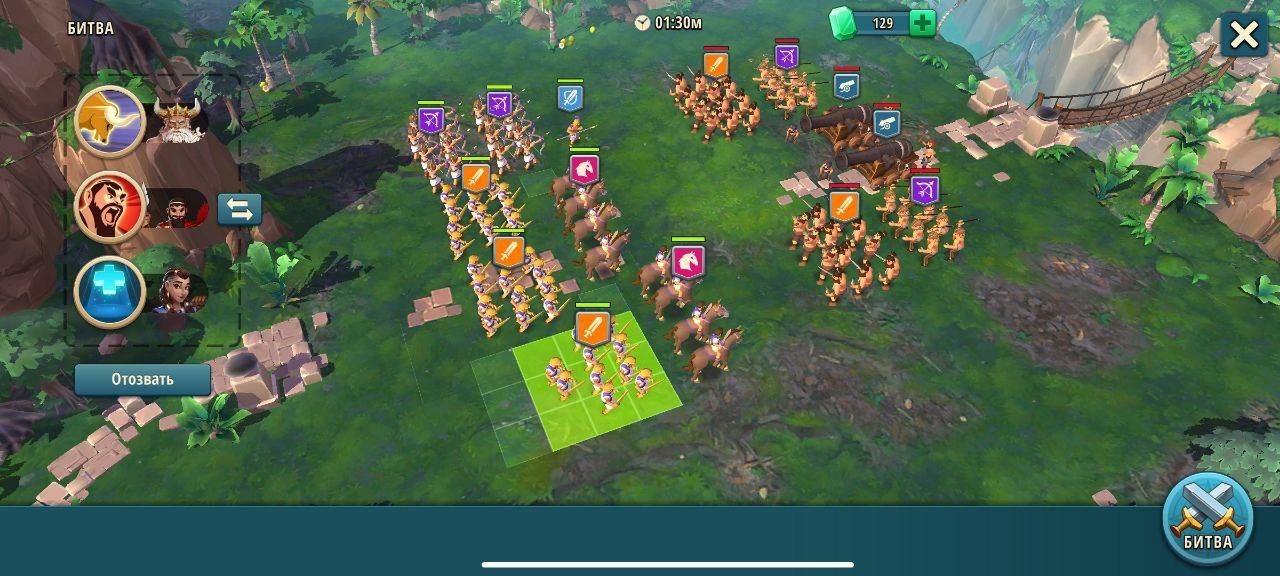
\includegraphics[width=\linewidth]{./parts/media/TreasureHunt/34/decoder/photo_2022-04-07_10-02-46.jpg} \newline
\noindent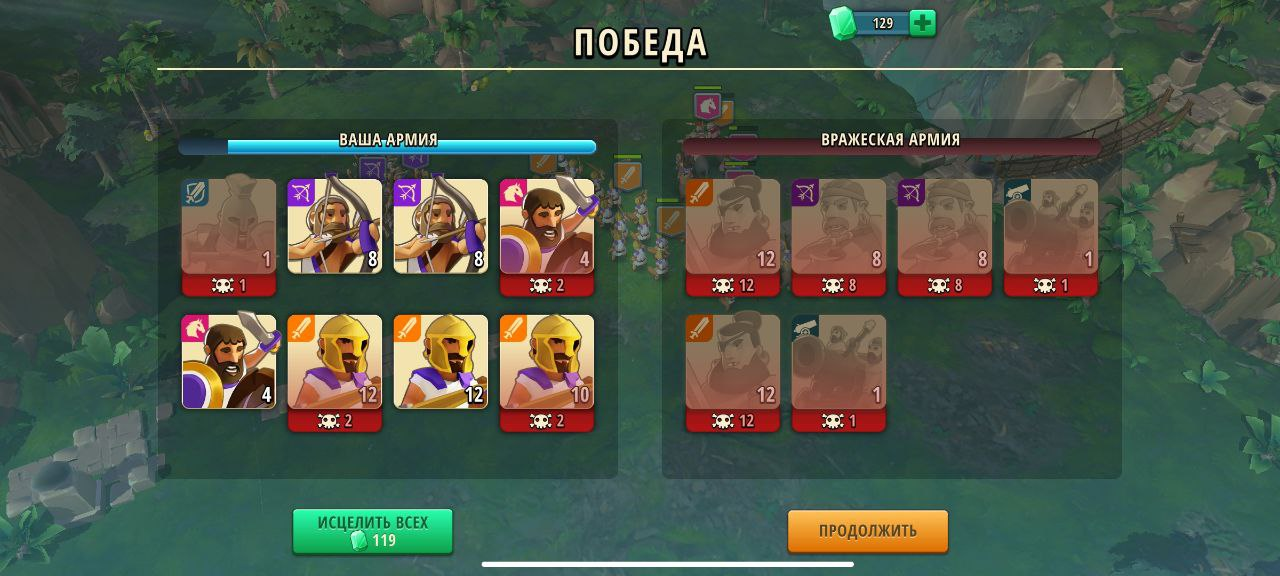
\includegraphics[width=\linewidth]{./parts/media/TreasureHunt/34/decoder/photo_2022-04-07_10-02-50.jpg} \newline

\newpage
\begin{center}
	\hypertarget{fight35}{\textbf{Битва 35 (Sargon).}}
\end{center}
\noindent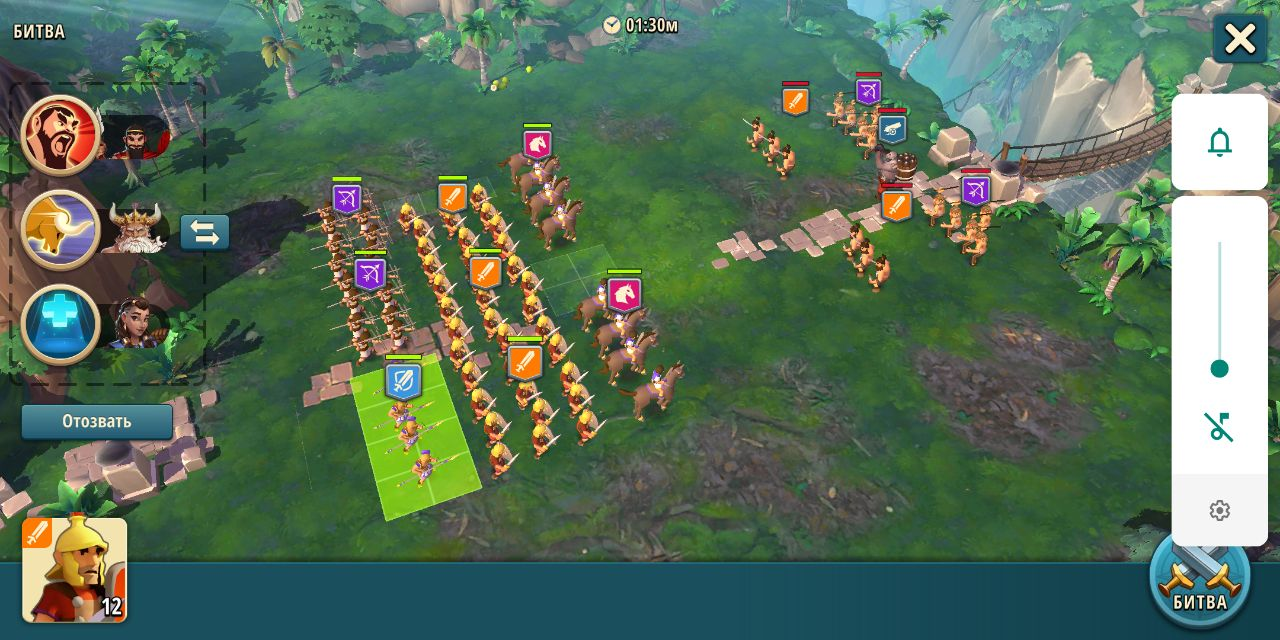
\includegraphics[width=\linewidth]{./parts/media/TreasureHunt/35/sargon/photo_2022-04-07_10-08-33.jpg} \newline
\noindent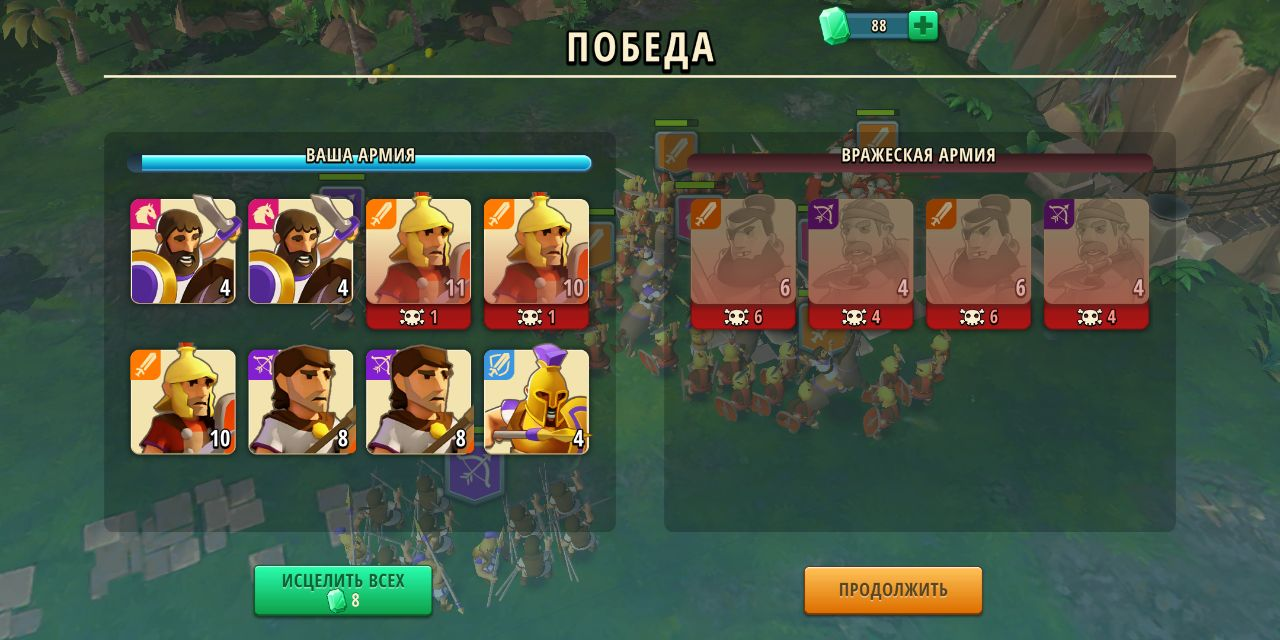
\includegraphics[width=\linewidth]{./parts/media/TreasureHunt/35/sargon/photo_2022-04-07_10-08-48.jpg} \newline
\noindent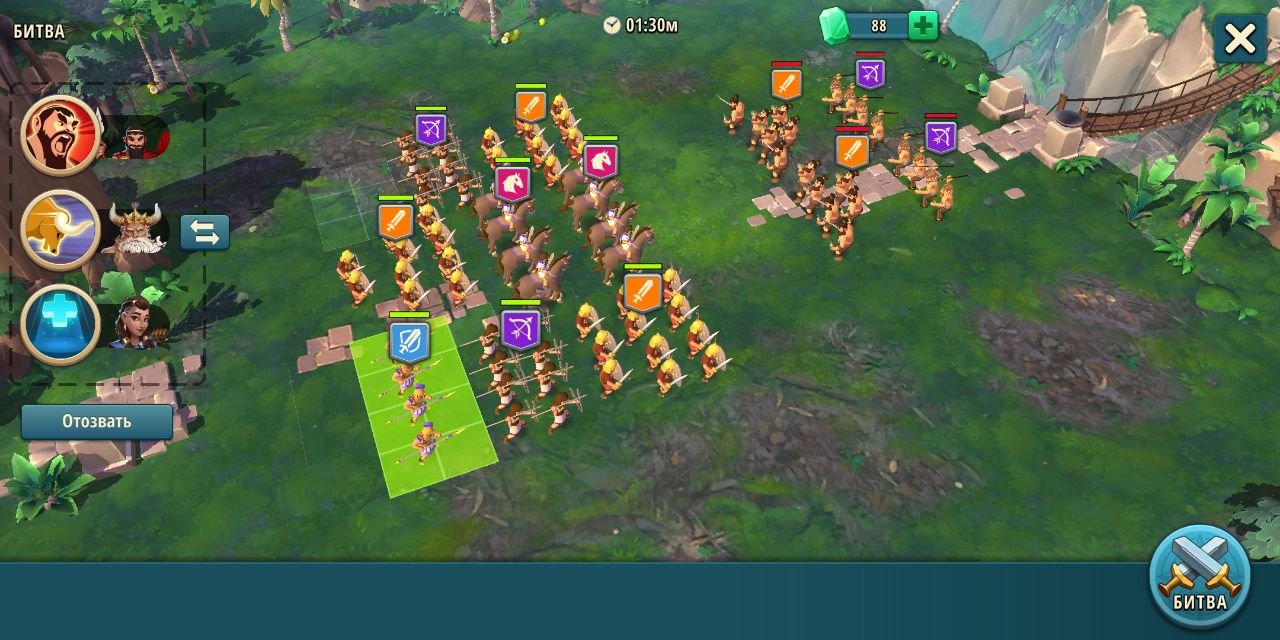
\includegraphics[width=\linewidth]{./parts/media/TreasureHunt/35/sargon/photo_2022-04-07_10-08-45.jpg} \newline
\noindent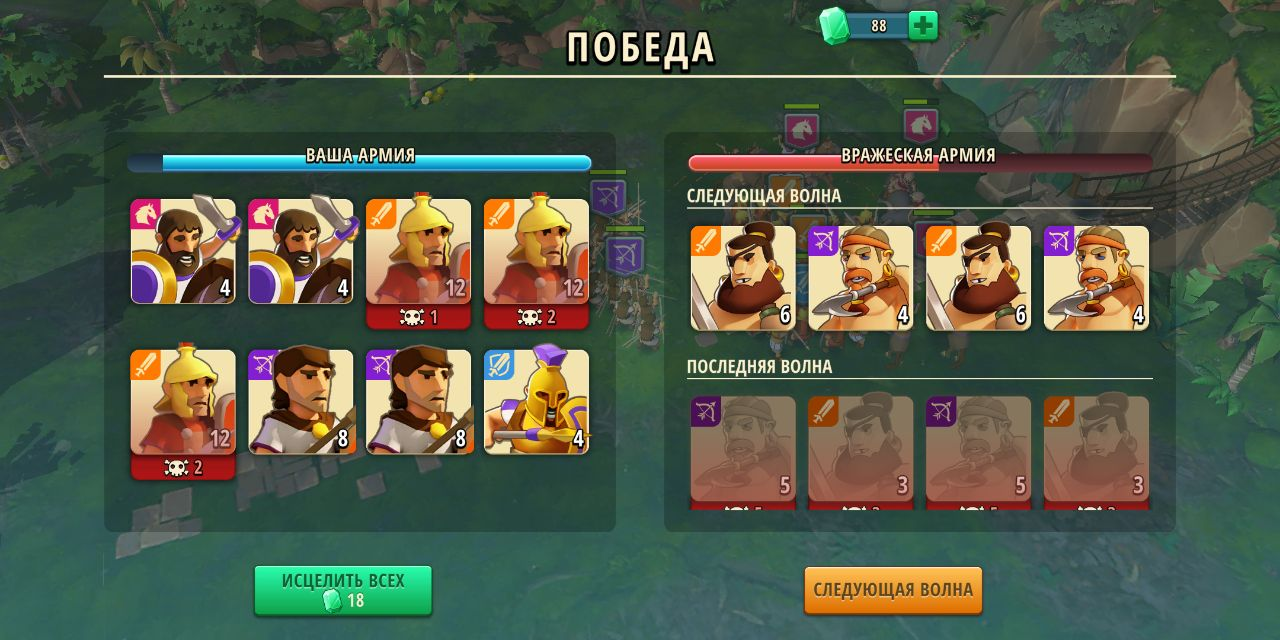
\includegraphics[width=\linewidth]{./parts/media/TreasureHunt/35/sargon/photo_2022-04-07_10-08-41.jpg} \newline

\newpage
\begin{center}
	\hypertarget{fight36}{\textbf{Битва 36 (Sargon).}}
\end{center}
\noindent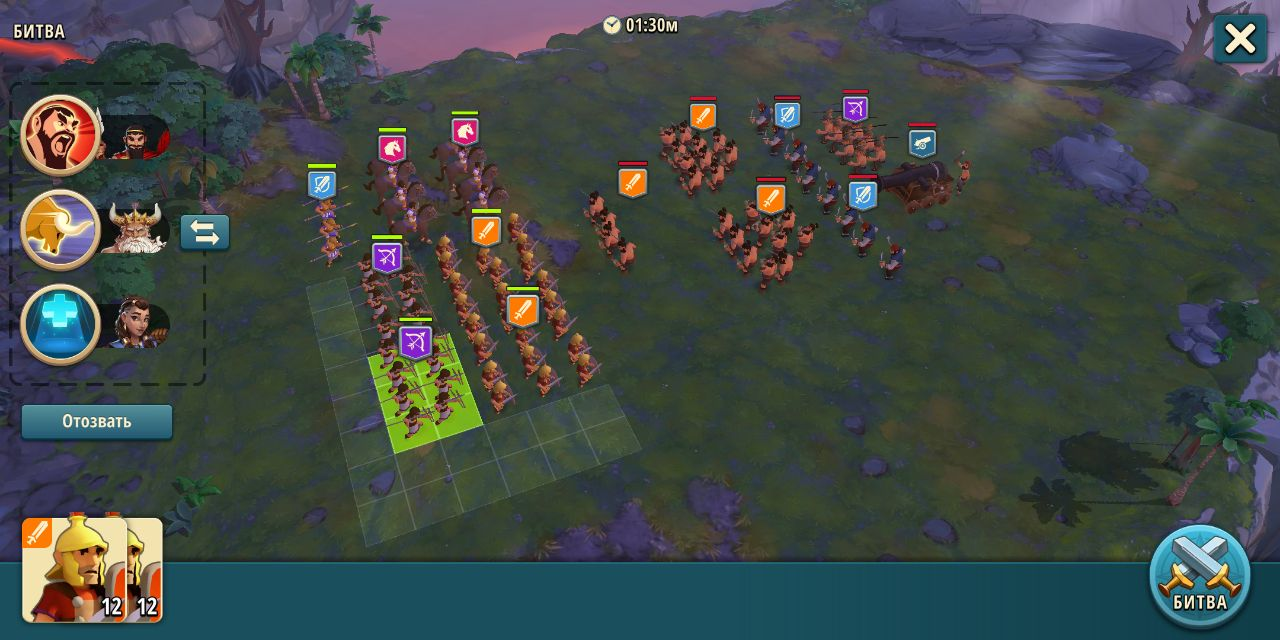
\includegraphics[width=\linewidth]{./parts/media/TreasureHunt/36/sargon/photo_2022-04-07_13-16-23.jpg} \newline
\noindent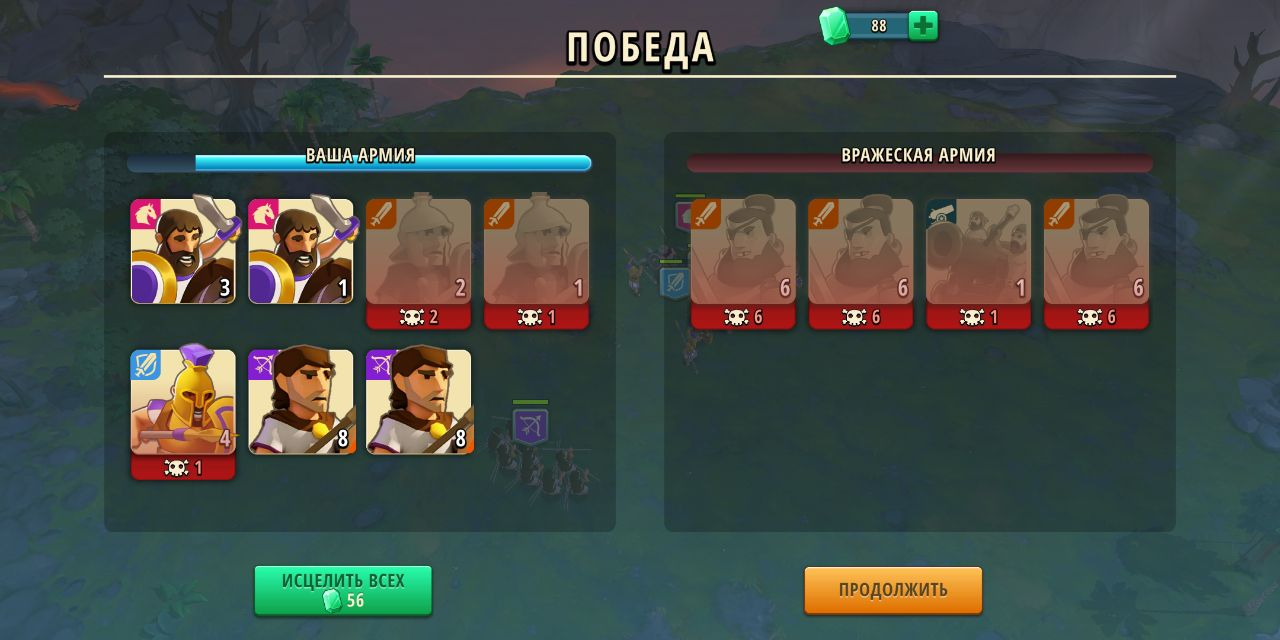
\includegraphics[width=\linewidth]{./parts/media/TreasureHunt/36/sargon/photo_2022-04-07_13-16-46.jpg} \newline
\noindent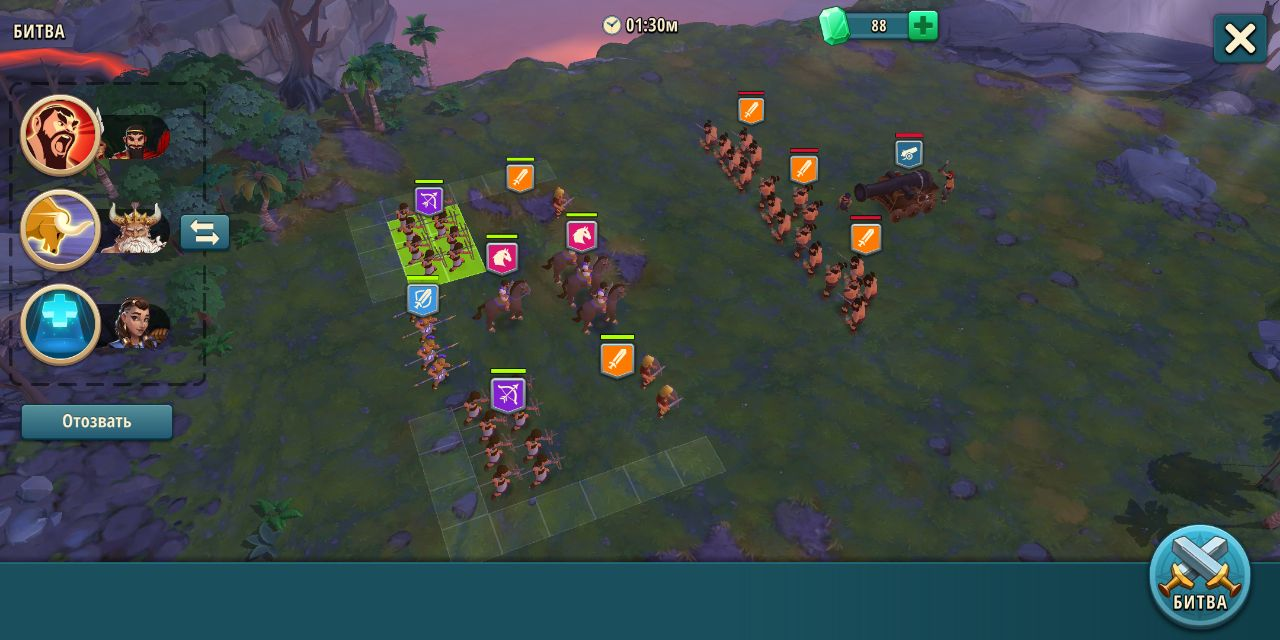
\includegraphics[width=\linewidth]{./parts/media/TreasureHunt/36/sargon/photo_2022-04-07_13-16-43.jpg} \newline
\noindent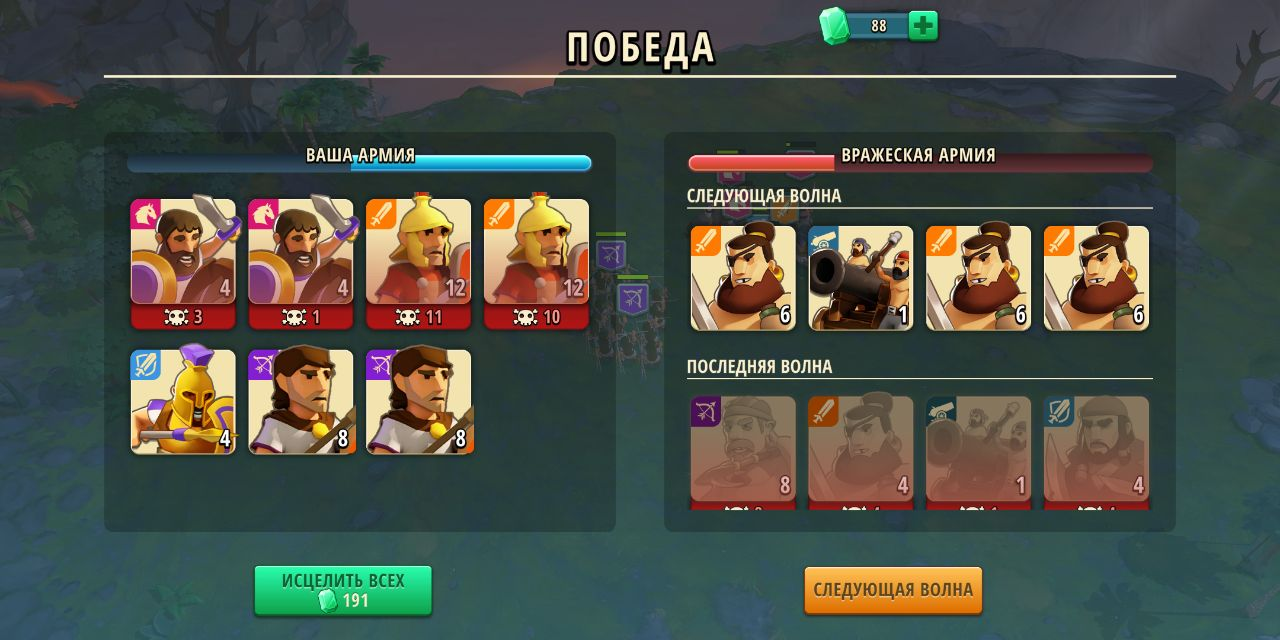
\includegraphics[width=\linewidth]{./parts/media/TreasureHunt/36/sargon/photo_2022-04-07_13-16-40.jpg} \newline

\newpage
\begin{center}
	\hypertarget{fight37}{\textbf{Битва 37 (decoder).}}
\end{center}
\noindent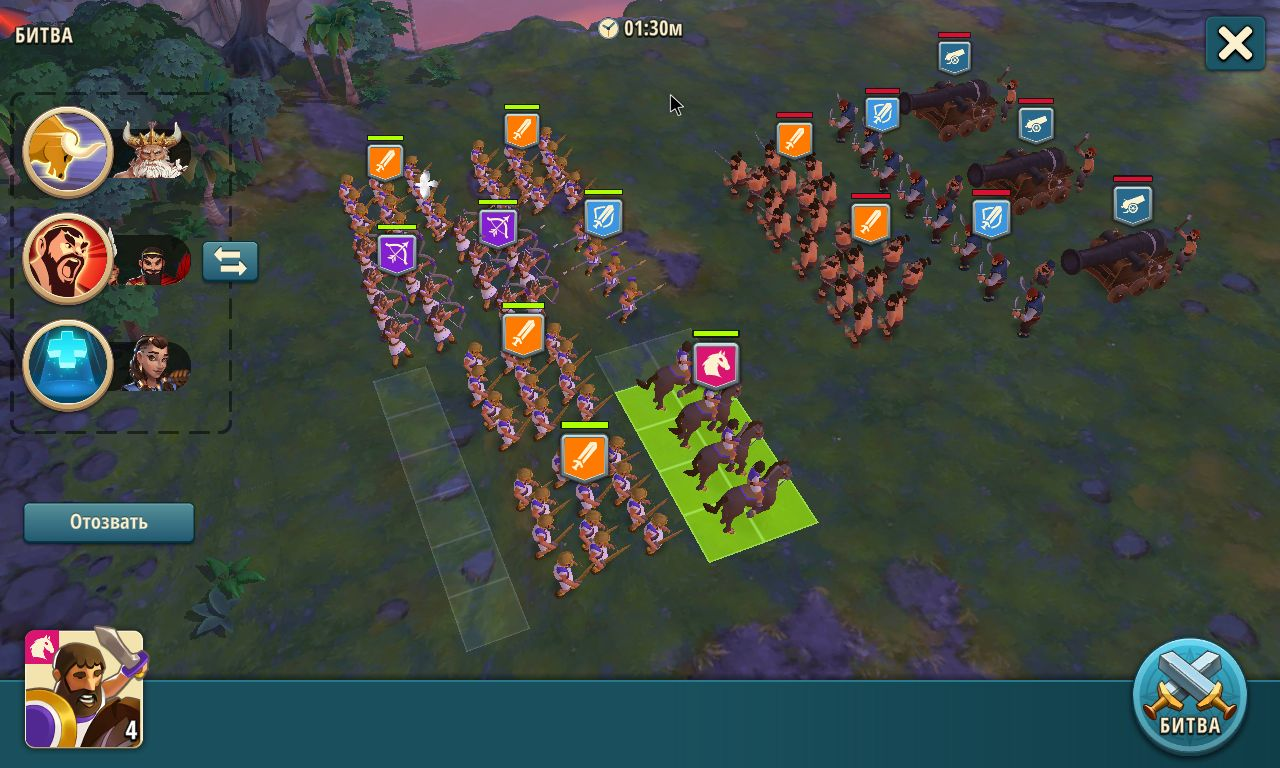
\includegraphics[width=\linewidth]{./parts/media/TreasureHunt/37/decoder/photo_2022-04-14_12-36-24.jpg} \newline
\noindent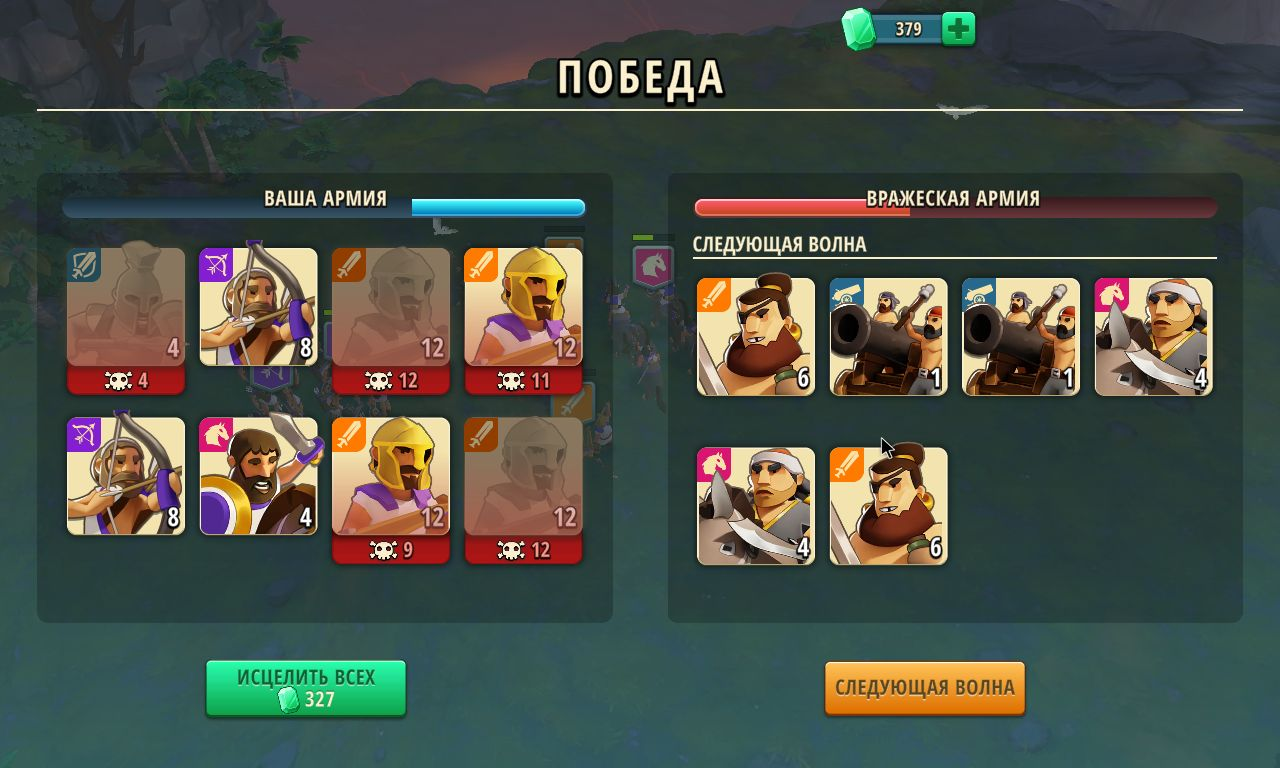
\includegraphics[width=\linewidth]{./parts/media/TreasureHunt/37/decoder/photo_2022-04-14_12-36-38.jpg} \newline
\noindent\includegraphics[width=\linewidth]{./parts/media/TreasureHunt/37/decoder/photo_2022-04-14_12-36-42.jpg} \newline
\noindent\includegraphics[width=\linewidth]{./parts/media/TreasureHunt/37/decoder/photo_2022-04-14_12-36-46.jpg} \newline

\newpage
\begin{center}
	\hypertarget{fight38}{\textbf{Битва 38 (Preyton).}}
\end{center}
\noindent\includegraphics[width=\linewidth]{./parts/media/TreasureHunt/38/Preyton/38.1.jpg} \newline
\noindent\includegraphics[width=\linewidth]{./parts/media/TreasureHunt/38/Preyton/38_1.jpg} \newline
\noindent\includegraphics[width=\linewidth]{./parts/media/TreasureHunt/38/Preyton/38.2.jpg} \newline
\noindent\includegraphics[width=\linewidth]{./parts/media/TreasureHunt/38/Preyton/38_2.jpg} \newline

\newpage
\begin{center}
	\hypertarget{fight39}{\textbf{Битва 39 (Sargon).}}
\end{center}
\noindent\includegraphics[width=\linewidth]{./parts/media/TreasureHunt/39/sargon/photo_2022-04-07_13-18-09.jpg} \newline
\noindent\includegraphics[width=\linewidth]{./parts/media/TreasureHunt/39/sargon/photo_2022-04-07_13-18-21.jpg} \newline
\noindent\includegraphics[width=\linewidth]{./parts/media/TreasureHunt/39/sargon/photo_2022-04-07_13-18-26.jpg} \newline
\noindent\includegraphics[width=\linewidth]{./parts/media/TreasureHunt/39/sargon/photo_2022-04-07_13-18-31.jpg} \newline

\newpage
\begin{center}
	\hypertarget{fight40}{\textbf{Битва 40 (decoder).}}
\end{center}
\noindent\includegraphics[width=\linewidth]{./parts/media/TreasureHunt/40/decoder/photo_2022-04-07_13-15-51.jpg} \newline
\noindent\includegraphics[width=\linewidth]{./parts/media/TreasureHunt/40/decoder/photo_2022-04-07_13-16-08.jpg} \newline
\noindent\includegraphics[width=\linewidth]{./parts/media/TreasureHunt/40/decoder/photo_2022-04-07_13-16-12.jpg} \newline
\noindent\includegraphics[width=\linewidth]{./parts/media/TreasureHunt/40/decoder/photo_2022-04-07_13-16-15.jpg} \newline
